\documentclass[12pt]{article}
\usepackage{graphicx,amssymb,amsmath,subfigure}

\oddsidemargin  -0.5 cm
\evensidemargin 0.0 cm
\textwidth      6.5in
\headheight     0.0in
\topmargin      -1 cm
\textheight=9in

\renewcommand{\arraystretch}{1.25}

\title{Global Alignment of the CMS Muon System \\ with Tracks using an Extended HIP Algorithm}
\author{Jim Pivarski, Alexei Safonov, Karoly Banicz, Riccardo Bellan}

\begin{document}
\maketitle
\begin{abstract}
We describe a track-based muon system alignment system using an
extended HIP algorithm.  We present the details of the procedure and
its validation with Monte Carlo simulation studies and discuss
data-driven monitoring and verification of alignment results.  We
applied this procedure to align the muon system with cosmic ray data
taken in 2008, and a variant of the procedure with beam-halo muons
from the 2008 LHC run, and present the results here.
\end{abstract}
\pagebreak

\tableofcontents
\pagebreak

\section{Introduction}

The CMS experiment features a large muon tracking system which will be
essential for early LHC discoveries.  As with all tracking systems,
the resolution of its reconstructed tracks depends on two main
components:
\begin{itemize}
\item intrinsic hit resolution, or how precisely the intersection of
  passing particles with its measurement planes can be determined for
  individual tracks, and
\item alignment, or how accurately the position of the measurement
  planes are known in 3-D space, affecting all tracks.
\end{itemize}
These components combine in quadrature, so track resolution can be
expected to improve significantly until the alignment is much better
than the intrinsic resolution, which is about 200--300~$\mu$m for the
CMS muon system.  Therefore, our baseline goal for the 2009--2010
physics run is to align the muon system to this level of accuracy.

Though this 44-layer muon system can act as a tracking system on its
own, it was designed to operate in conjunction with the other CMS
subsystems, particularly the inner silicon tracker.  Together, the two
tracking subsystems form a global tracking system with high intrinsic
hit resolution in the tracker and large lever arm in the muon system
(particularly important for high-$p_T$ tracks; $1/p_T$ resolution
scales with the length of the usable radial lever arm squared).  Above
$p_T \gtrsim 200$~GeV in the barrel and 1~TeV in the endcap, the
inclusion of muon system hits significantly improves muon resolution
over a tracker-only measurement (Fig~\ref{fig:tdr_muon_resolution}).
Muon alignment is therefore important for any physics analysis
featuring high-$p_T$ muons, such as $Z' \to \mu\mu$ and $W' \to
\mu\nu$, but it is also important for analyses that use the muon
system as an independent check on the tracker, such as the search for
heavy stable charged particles, which verifies velocity from tracker
$dE/dx$ with muon barrel timing (equivalent to spatial resolution).

\begin{figure}[hb]
\begin{center} \includegraphics[width=0.35\linewidth]{Figure_001-005-a.pdf} \hspace{0.5 cm} \includegraphics[width=0.35\linewidth]{Figure_001-005-b.pdf} \end{center}
\caption{Momentum resolution of the inner tracker, muon system, and combined system, as a function of $p_T$ and $\eta$.  (Source: Physics TDR~\cite{tdr}) \label{fig:tdr_muon_resolution}}
\end{figure}

To obtain high-quality global muon tracks, the tracker and muon system
must be aligned in the same coordinate system.  We choose to define
the global coordinate system as the inner tracker's system and verify
that it is stable for each block of runs.  This is convenient because
the low-momentum tracks used to measure the alignment (20--100~GeV)
are best determined by the tracker.  If a sudden movement or slow
drift is observed, we have the necessary machinery to redefine the
global coordinate system in a more neutral way.

There are several independent ways to measure alignment, all of which
are actively being pursued.  Alignment with global muon tracks
provides a simple way to link distant subdetector elements and is
sensitive to exactly the same parameters as the muon tracks used in
physics analyses.  For example, if misalignment perpendicular to the
measurement plane of a layer cannot be determined from a large sample
of tracks, then it also does not distort the physics resolution of
muons in the same sized sample.  Alignment with local tracks, such as
linear track stubs through pairs of neighboring detector elements, can
determine the relative positions of those elements and provide both an
early (low statistics) alignment measurement and a powerful
cross-check on the global alignment, as local tracks are much less
sensitive to propagation errors and have a different pattern of
correlations.  The CMS muon system is also instrumented with a network
of physical measurement devices such as lasers, calipers, and
inclinometers, which provide another independent measurement of
detector alignment, free from any tracking errors but requiring a
careful propagation of cumulative measurements.  This paper will focus
on alignment with global tracks for both the barrel and the endcap,
and demonstrate an alignment procedure with local tracks in the
endcap.

\subsection{Geometry of the muon system}

The muon system contains three basic types of tracking chambers: drift
tube (DT) chambers in the barrel, cathode strip chambers (CSC) in the
endcap, and resistive plate chambers (RPC) in both.  The chambers are
modular tracking detectors, 1--4~m each, whose internal geometry is
well understood from production tests.  They are mounted on 15~m tall
barrel wheels and endcap disks which serve to compactly return the
solenoid's magnetic field and also filter all particles except for
muons.  The position and orientation of each chamber is allowed to
slip under the influence of the 3.8~T CMS solenoid, rather than
distort the chambers non-rigidly.  In the center of the endcap, this
distortion can be as large as 1.4~cm.

This paper focuses on algorithms to align the DT chambers and CSCs as
rigid bodies whose internal geometry is assumed to be known.  The DT
internal geometry has been thoroughly studied elsewhere
\cite{internal_dt}, and a method to align CSC layers will be described
in section~\ref{sec:CSC_layer_alignment}.  The RPCs are used primarily
for triggering with a resolution of 1--2~cm, so they do not contribute
to muon resolution and do not need to be aligned regularly.

The chambers are grouped in stations (loosely by distance from the
interaction point), wheels/disks (modular transverse slices), and
sectors/chambers (azimuthal divisions).  Table~\ref{tab:geometry} presents an
overview of this structure, and Fig~\ref{fig:muon_system_labeled}
shows where the stations are located in CMS.

\begin{table}
\caption{Geographical organization of muon chambers. \label{tab:geometry}}
\begin{center}
\begin{tabular}{c | c}
Barrel & Endcap \\\hline
\renewcommand{\arraystretch}{2.5}
\begin{tabular}{p{0.08\linewidth} p{0.125\linewidth} p{0.13\linewidth}}
wheels & $-2$ to $+2$ & physically moveable transverse slices \\
stations & MB1 to 4 & cylinders of fixed radius from beamline \\
sectors & 1--12 \mbox{(1--14 in} station~4) & \raggedright $\phi=0$ is sector 1, increasing counter-clockwise \\
\end{tabular} &
\begin{tabular}{p{0.1\linewidth} p{0.125\linewidth} p{0.14\linewidth}}
endcaps & $-$ and $+$ & forward and backward halves \\
disks & ME1 to 4 & physically moveable transverse slices \\
rings \mbox{(stations)} & \raggedright 1/1ab, 1/2, 1/3, 2/1, 2/2, 3/1, 3/2, 4/1 & rings of fixed radius from beamline \\
chambers & 1--36 \raggedright \mbox{(1--18 in} 2/1, 3/1, 4/1) & \raggedright $\phi=0$ is sector 1, increasing counter-clockwise \\
\end{tabular}
\vspace{-1 cm}
\end{tabular}
\end{center}
\end{table}

\begin{figure}
\hspace{-1.3 cm} \includegraphics[width=1.2\linewidth]{muon_system_labeled.pdf}

\caption{A quarter-view of CMS with labeled muon barrel (MB) and endcap (ME) stations. \label{fig:muon_system_labeled}}
\end{figure}

The CMS global coordinate system is defined with respect to the LHC
beamline: the $+z$ direction points along the beamline, to the west.
The $+y$ axis is vertically upward, with $+x$ forming a right-handed
coordinate system by pointing south, toward the center of the LHC
ring.  The same coordinates can be expressed cylindrically, with $x$
and $y$ replaced by $r = \sqrt{x^2 + y^2}$ and $\phi = \mbox{atan2}(y,
x)$, which is often more natural given CMS's near-cylindrical
symmetry~\cite{CMSConventions}.  We use the curvilinear coordinate
$r\phi$ to denote a direction perpendicular to $z$ and $r$, at a given
$r$, in units of length.  Differentials of $r\phi$
(e.g.\ $d(r\phi)/dz$) vary in $\phi$, not $r$ (so they are equivalent
to $r \, d\phi/dz$).

Each muon chamber and layer has its own local coordinate system,
centered on the subdetector with local $z$ being perpendicular to the
measurement plane.  The local $x$ direction is always the direction
measured with highest precision, arranged to coincide with global
$r\phi$, and local $y$ forms a right-handed coordinate system.  In
barrel stations 1--3, DT chambers measure $x$ and $y$ with different
superlayers: superlayers 1 and 3 measure local $x$ coordinates and
superlayer 2 (located between 1 and 3) measures local $y$, roughly
parallel with the beamline.  In the absence of misalignment, the DT
local $y$ axis is exactly parallel with global $z$.  Barrel station~4
chambers have no superlayer~2, so they can not measure $y$ positions
of hits.

In the CSCs, cathode strips fan radially from the beamline,
intersected by anode wires.  The strips measure a coordinate
perpendicular to their orientation, differing from global $r\phi$ only
due to misalignment.  The local cartesian $x$ direction is parallel
with the strip measurement in the center of the chamber, and $y$ is
roughly radial.  In the CSCs, local $z$ is parallel with global $z$,
differing in sign for half of the chambers.
Table~\ref{tab:local_coordinates} summarizes all of these coordinate
systems.

Layer coordinate systems differ from their parent chamber's in only
three ways: they have a different origin, with $z=0$ being centered on
the physical measurement plane, DT superlayer~2 is rotated 90$^\circ$,
and layers may require small alignment corrections.  Hit positions are
measured in the layer coordinate system, and must be transformed to
the chamber system when calculating chamber corrections, particularly
angles, since these are defined with respect to the chamber's center.

\begin{table}
\caption{Definitions and correspondance of coordinate systems. \label{tab:local_coordinates}}
\begin{center}
\begin{tabular}{c | c | c}
Global frame & Local DT frames & Local CSC frames \\\hline
\begin{tabular}{c p{0.2\linewidth}}
$x$ & horizontal, toward center of LHC \\
$y$ & vertical, up \\
$z$ & along beamline \\
origin & nominal interaction point \\
$r\phi$ & combination of $x$ and $y$ perpendicular to
rays from the beamline
\end{tabular} &
\begin{tabular}{c p{0.2\linewidth}}
$x$ & superlayer~1 and 3 measurement, roughly global $r\phi$ \\
$y$ & superlayer~2 measurement, roughly global $z$ \\
$z$ & out of plane, roughly radial from beamline \\
origin & center of chamber
\end{tabular} &
\begin{tabular}{c p{0.2\linewidth}}
$x$ & strip measurement, roughly global $r\phi$ \\
$y$ & wire measurement, roughly radial from beamline \\
$z$ & out of plane, roughly global $z$ \\
origin & center of chamber
\end{tabular}
\end{tabular}

\vspace{0.25 cm}
$\phi_x$, $\phi_y$, and $\phi_z$ are rotation angles around local
coordinate axes.

\end{center}
\end{table}

\section{Description of the global alignment algorithm}

The basic idea is to accumulate high-$p_T$ muons which pass through
two regions: a well-aligned ``Reference'' volume, usually the silicon
tracker, and the ``Target'' volume under study.  Muon tracks are
fitted using information from the Reference only, and alignables in
the Target (muon chambers, layers, wheels, or disks) are translated
and rotated to minimize the difference between muon hits and the
intersection of tracks with the layer planes (residuals).

This procedure can be seen as an extreme limit of the HIP algorithm
(``Hits and Impact Points,'' where impact points are the track
intersections) used to align the silicon tracker~\cite{trackerhip}, in
which tracks are fitted in a single tracking volume with large
uncertainties in the positions of the alignables.  The uncertainties
reduce the sensitivity of the final track fits to outlying alignables,
so that these alignables will have larger residuals.  Those residuals
may be biased and not represent the whole misalignment, but repeated
applications of the procedure draws alignables closer to their
rightful positions and finally converges when a fully consistent
system is reached.

In comparison with the silicon tracker case, however, individual
tracks propagated through the muon system are much less trustworthy
due to the large amounts of material they must penetrate.  Muons,
particularly low-momentum muons, can be highly deflected by the single
and multiple scattering which occurs unpredictably in dense material,
and can distort the track-fit if not recognized by the algorithm.
CMS's Kalman track-fitting algorithm properly includes such
scattering, but as a by-product, tracks fitted to misaligned chambers
can be misinterpreted as scattering in the iron before entering the
chamber.  Each Kalman track-fit is performed independently, so the
systematic nature of misalignment would be ignored, biasing all tracks
in the sample.  By instead propagating the tracks from the Reference
volume through the Target, not allowing Target hits to refine the
propagated track, only the muons that actually do scatter
significantly are useless for alignment.

The technique is particularly useful when the Reference volume is the
silicon tracker, since the tracker dominates the precision of track
parameters for the muons used in alignment ($20 < p_T < 100$~GeV).
The disadvantage is that any distortions in the tracker geometry,
which can persist after completing tracker alignment if the $\chi^2$
of its tracks are invariant under such transformations, would be
extrapolated to the muon system, distorting the muon geometry in the
same way.  However, the broad track angle distribution of cosmic rays
allows us to observe residuals on tracks from different parts of the
Reference volume, and therefore put bounds on the bias from the track
source.  The tracker alignment procedure uses this same technique to
constrain its ``weak modes,'' but the muon system provides additional
checks with a longer lever arm, to amplify the errors and more easily
notice the effects.

It is also a computationally useful feature that excluding Target hits
from the track-fit eliminates the coupling between track-fitting and
alignment.  We therefore do not need to iterate the procedure, as in
the case in the tracker-HIP alignment, because geometry updates in the
Target have no effect on track-fitting in the Reference.  In the
language of MillePede-based algorithms, the matrix of alignment
parameters and track parameters becomes block-diagonal, greatly
simplifying its inversion and eliminating the fundamental distinction
between the HIP and MillePede approaches.

\subsection{Alignment datasets and track-fitting procedures}

Data used for muon HIP alignment are derived from three main sources:
LHC collisions, cosmic rays that pass through the tracker, and cosmic
rays that do not pass through the tracker.  The main difference
between the three datasets is the pattern of chambers and tracker
silicon wafers they connect.  An alignment procedure may be
represented by a graph of Reference and Target detector elements (the
vertices of the graph) connected by tracks (the edges).  Tracks
measure the relative positions of the detector elements they connect,
and loops in the graph provide consistency checks to confirm that
relative positions are transitive (as they must be if they represent
true positions in space).  Muons from LHC collisions always pass
through nearly the same set of detector elements, so they connect
silicon wafers to muon chambers as a directed tree.  If the silicon
wafers that ``point'' to a given muon chamber are coherently
misaligned, this misalignment would be propagated to the muon chamber.

Cosmic rays do not originate from a point source, so they connect muon
chambers to silicon wafers in a more complicated mesh with many loops.
Each muon chamber recieves cosmic rays from a variety of paths through
the tracker, effectively averaging over any residual misalignments in
it.  The disadvantage of cosmic rays is that their distribution is
highly non-uniform, with a hit distribution peaking steeply at the top
and bottom of the detector, especially if these cosmic rays are also
required to pass through the tracker.  Cosmic rays that do not pass
through the tracker have a more inclusive distribution, but lack a
high-precision Reference.  It should also be noted that the number of
cosmic ray muons ($\mu^-$) is not equal to the number of cosmic ray
antimuons ($\mu^+$), especially in regions of the detector where one
sign of curvature points inward, toward more detector elements, and
the other points outward.  Some tracking biases affect $\mu^-$ tracks
differently than $\mu^+$ tracks, a point which we will consider in
more detail later.

The production mechanism of our collisions muons does not need to be
controlled, only the $p_T$ distribution.  Whether a muon was the
product of a $b$ decay or a $Z$ decay, its propagation through the
tracker and muon system is determined solely by its momentum.  We
therefore only require one muon in the event, with
20~GeV$<$~$p_T$~$<$~100~GeV.  The lower limit excludes tracks that are
likely to scatter and the upper limit guarantees that track parameters
are well determined by the tracker.  The muons selected this way are
primarily from heavy flavor sources, and the spectrum is steeply
peaked at low momentum.

The events are collected by AlCaReco producers (fully-Reconstructed
formats for Alignment and Calibration), which select good muon tracks
in prompt reconstruction at CERN's Tier-0 computing center, reduce the
data streams to include only the needed tracks and hits, and send them
to the CMS CAF (Computing Analysis Farm) to be persistently stored on
a local disk.  The AlCaReco stream for collisions muons is named
MuAlCalIsolatedMu (though no isolation requirements are applied), the
stream for cosmics that pass through the tracker is MuAlGlobalCosmics
(because they are combined into global tracks with both tracker and
muon hits), and the stream for the rest of the cosmic rays is
MuAlStandAloneCosmics (stand-alone tracks are reconstructed in the
muon system only)\label{page:AlCaReco}.

The first step in the alignment algorithm is to re-fit the tracks,
using the original track parameters to seed the new fit.  This allows
us to take advantage of any updates in the Reference geometry and to
include artificially large chamber position uncertainties in the
Target hit positions (1000~cm, isotropically in $x$-$y$-$z$).  The
Target hits are technically included in the track re-fit, but the
large uncertainty makes them effectively ignored, with nearly zero
pull in the fit.  The advantage of this method over simply dropping
the Target hits is that residuals are calculated using the same
routines as standard track-fitting, inheriting any bug-fixes included
in standard tracking.  These chamber position uncertainties (called
Alignable Position Errors, or APEs) are expressed in a mutable
database record, so the boundary between the Reference and Target
volumes can be arbitrarily defined.

In performing the track re-fit, it is essential that the algorithm
starts with the Reference hits and ends with the target hits;
otherwise, the new track's trajectory through the Target will be
determined by the old seed track, rather than a new fit to the
Reference.  For collisions muons, this means that fitting must be
performed in the direction of muon momentum (``alongMomentum'' or
``insideOut''), and for cosmic rays, two specialized refitters,
globalCosmicMuonTrajectories and standAloneMuonTrajectories, have been
written to set the hit order in a reliable way.  The
globalCosmicMuonTrajectories algorithm arranges hits to start in the
tracker and end in the muon system, while standAloneMuonTrajectories
requires the first hit to be closest to the center of CMS (in global
$z$) and the last to be farthest.  Thus Reference volumes in the muon
system must always include the central barrel wheel (wheel~0):
alignment knowledge is propagated from wheel~0 out to the endcaps.

\subsection{Calculation of super-residuals}
\label{sec:super_residuals}

As a tracking volume, the muon system is highly structured.  Inside of
each chamber, muons encounter negligible material, and in the barrel
chambers, also very little magnetic field.  Between chambers, muons
pass through thick, magnetized iron and potentially change direction
due to scattering.  Individual muon hits are therefore more highly
correlated with their neighbors in the same chamber than they are with
the paths of propagated tracks.  We find it useful to combine all
residuals in each chamber on each track into a ``super-residual''
representing the difference in position and angle between the
propagated track and all of the hits.

Ignoring the correlation between residuals would lead to an improper
treatment of statistics.  For the sake of argument, consider an
extreme case in which residuals in an $N$-layer chamber are 100\%
correlated with each other (no intrinsic error).  If we accumulate a
histogram of residuals for that chamber, each track will yield the
same result $N$ times, though the distribution would be determined by
the uncertainties in track propagation.  If we then compute the mean
of that distribution or fit it, the reported uncertainties would be a
factor of $\sqrt{N}$ too small.

A super-residual is an analytic linear fit to all residuals in one
chamber on one track (Fig~\ref{fig:superresidual0}).  It is expressed
in the chamber's local coordinate system, in which each hit lies on a
layer of fixed $z_i$, with $z=0$ being the chamber's center.  Denoting
the individual residuals as $\Delta x_i$ and the corresponding hit
uncertainties as $\sigma_i$, the super-residual position $\Delta x$
and angle $\Delta \frac{dx}{dz}$ are

\begin{figure}
\begin{center} 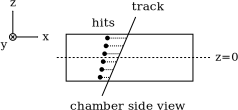
\includegraphics{superresidual2.pdf} \end{center}
\caption{A super-residual has two or four components: the slope of individual $x$ residuals versus the $z$ positions of their layers ($\Delta \frac{dx}{dz}$), their intercept at $z=0$ ($\Delta x$), and the same for $y$ residuals, if measured. \label{fig:superresidual0}}
\end{figure}

\begin{eqnarray}
\Delta x &=& \frac{1}{\mbox{denominator}} \left(\sum\frac{z_i^2}{\sigma_i^2} \sum\frac{\Delta x_i}{\sigma_i^2} - \sum\frac{z_i}{\sigma_i^2} \sum\frac{z_i \Delta x_i}{\sigma_i^2}\right) \\
\Delta \frac{dx}{dz} &=& \frac{1}{\mbox{denominator}} \left(\sum\frac{1}{\sigma_i^2} \sum\frac{z_i \Delta x_i}{\sigma_i^2} - \sum\frac{z_i}{\sigma_i^2} \sum\frac{\Delta x_i}{\sigma_i^2}\right) \\
\mbox{where denominator} &=& \sum\frac{1}{\sigma_i^2} \sum\frac{z_i^2}{\sigma_i^2} - \left(\sum\frac{z_i}{\sigma_i^2}\right)^2\mbox{.}
\label{eqn:super-residual}
\end{eqnarray}
Chambers that are capable of measuring local $y$ positions of hits
have a super-residual $\Delta y$ and $\Delta \frac{dy}{dz}$ defined
the same way.

Note that this differs from simply averaging the residuals, because the
fit guarantees that $\Delta x$ and $\Delta y$ represent the difference
between the track propagation and chamber measurement at the chamber
origin ($z=0$).  It also differs from ``segment residuals,'' in which
the raw hit positions are fitted to a straight line instead of hit
residuals.  A segment residual injects the assumption that tracks
propagate linearly through the chamber, while a super-residual only
assumes that small errors grow linearly.  This is particularly
important for chambers immersed in a large magnetic field, such as
ME1/1 and ME1/2.

Each super-residual also has a corresponding quality-of-fit parameter
\begin{equation}
\chi^2/\mbox{ndf} = \frac{1}{N - 2} \sum \frac{\left(x_i - \Delta x - \Delta \frac{dx}{dz} z_i\right)^2}{{\sigma_i}^2}
\end{equation}
which can be used to identify super-residuals containing spurious
hits.  Rather than applying a cut at an arbitrary $\chi^2/\mbox{ndf}$
value, we later use them as weights to prefer straight super-residuals
in alignment.  Super-residuals are, however, required to contain a hit
on every layer in the chamber.

DT super-residuals have four coordinates, $\Delta x$, $\Delta y$,
$\Delta \frac{dx}{dz}$, and $\Delta \frac{dy}{dz}$, except for
chambers in station~4.  Station~4 chambers have only $\Delta x$ and
$\Delta \frac{dx}{dz}$ because they lack a $y$-measuring superlayer~2.

CSC super-residuals are computed in a curvilinear coordinate system
with two coordinates, $\Delta r\phi$ and $\Delta \frac{d(r\phi)}{dz}$.
Angled strips measure residuals perpendicular to the strip angle
(Fig~\ref{fig:csc_localrphi}), a direction which roughly corresponds
to global $r\phi$.  Local $y$ positions, determined by anode wires,
are unreliable because they are ganged in groups as large as 5~cm,
much larger than the scale of misalignments.  Alignment depends
sensitively on the peak of a well-understood residuals distribution,
and the discretization in $y$ complicates that shape.  The CSC
super-residual coordinates are calculated using
Eqn~\ref{eqn:super-residual} with $\Delta x_i$ replaced by $\Delta
r\phi_i$, where the latter is the difference between track and hit in
the local direction perpendicular to the strip angle.  Alignment in a
curvilinear coordinate system has consequences that will be addressed
in the next section.

\begin{figure}
\begin{center} 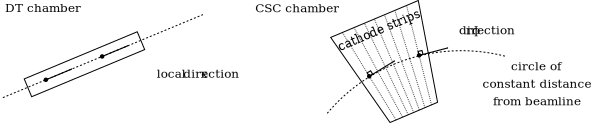
\includegraphics{strip_direction.pdf} \end{center}
\caption{Local $x$ and $y$ coordinates in DT chambers are rectilinear, but the fanning of CSC strips makes it more convenient to measure residuals and align CSCs in curvilinear $r\phi$. \label{fig:csc_localrphi}}
\end{figure}

\subsection{Differential geometry of super-residuals}

Super-residuals (henceforth simply referred to as ``residuals'')
quantify the misalignment of muon chambers because a small error in
the transformation from local hit positions to global hit positions
leads to systematic offsets between hits and unbiased tracks.  It is
useful to separate the geometric contribution, ${\Delta
  x}^{\mbox{\scriptsize geom}}$, from the measurement error, ${\Delta
  x}^{\mbox{\scriptsize meas}}$, a random variable centered on zero if
there is no bias.  The observed residuals distribution is the sum of
these two contributions.

Geometric residuals are a projection of the misalignment onto
${\Delta x}^{\mbox{\scriptsize geom}}$, ${\Delta y}^{\mbox{\scriptsize geom}}$,
${\Delta \frac{dx}{dz}}^{\mbox{\scriptsize geom}}$, and
${\Delta \frac{dy}{dz}}^{\mbox{\scriptsize geom}}$.  For some
misalignments, this projection is trivial: a 1~mm $\delta_x$
misalignment (in the chamber's local $x$ direction) does not affect
any residuals components except ${\Delta x}^{\mbox{\scriptsize geom}}$,
which is shifted by 1~mm.  Other misalignments, such as
$\delta_{\phi_z}$ and $\delta_z$ introduce
${\Delta x}^{\mbox{\scriptsize geom}}$ residuals which depend on the
track's intersection point $(x,y)$ and entrance angle $(\frac{dx}{dz},
\frac{dy}{dz})$ on the chamber (Fig~\ref{fig:phiz_zpos}).

\begin{figure}
\subfigure[Linear relationship between $\Delta x$ residuals, $\delta \phi_z$ misalignment, and $y$ track position: \mbox{${\Delta x}^{\mbox{\scriptsize geom}} = y \, \delta_{\phi_z}$}]{\begin{minipage}{0.4\linewidth} \begin{center} 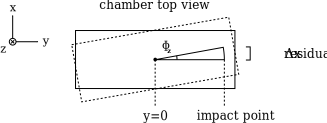
\includegraphics{phiz_diagram.pdf} \end{center} \vspace{0.2 cm} \end{minipage}} \hfill \subfigure[Linear relationship between $\Delta x$ residuals, $\delta z$ misalignment, and $dx/dz$ track angle: \mbox{${\Delta x}^{\mbox{\scriptsize geom}} = (dx/dz) \, \delta z$}]{\begin{minipage}{0.4\linewidth} \begin{center} 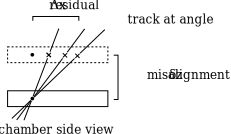
\includegraphics{zpos_diagram.pdf} \end{center} \vspace{0.2 cm} \end{minipage}}
\caption{Geometric relationships between $\delta_z$, $\delta_{\phi_z}$ misalignments and $\Delta x$ residuals. \label{fig:phiz_zpos}}
\end{figure}

In general, the transformation from rigid body misalignments
$\delta_x$, $\delta_y$, $\delta_z$, $\delta_{\phi_x}$,
$\delta_{\phi_y}$, and $\delta_{\phi_z}$ to residuals is given by the
following transformation:
\begin{equation}
\renewcommand{\arraystretch}{2.5}
\left(\begin{array}{c}
{\Delta x}^{\mbox{\scriptsize geom}} \\
{\Delta y}^{\mbox{\scriptsize geom}} \\
{\Delta \dfrac{dx}{dz}}^{\mbox{\scriptsize geom}} \\
{\Delta \dfrac{dy}{dz}}^{\mbox{\scriptsize geom}} \\
\end{array}\right)
=
{\renewcommand{\arraystretch}{2.5}
\left(\begin{array}{c c c c c c}
1 & 0 & -\dfrac{dx}{dz} & -y \dfrac{dx}{dz} & x \dfrac{dx}{dz} & -y \\
0 & 1 & -\dfrac{dy}{dz} & -y \dfrac{dy}{dz} & x \dfrac{dy}{dz} & x \\
0 & 0 & 0 & -\dfrac{dx}{dz} \dfrac{dy}{dz} & 1 + \left(\dfrac{dx}{dz}\right)^2 & -\dfrac{dy}{dz} \\
0 & 0 & 0 & -1 - \left(\dfrac{dy}{dz}\right)^2 & \dfrac{dx}{dz}\dfrac{dy}{dz} & \dfrac{dx}{dz}
\end{array}\right)}
\renewcommand{\arraystretch}{1.7}
\left(\begin{array}{c}
\delta_x \\
\delta_y \\
\delta_z \\
\delta_{\phi_x} \\
\delta_{\phi_y} \\
\delta_{\phi_z}
\end{array}\right) \mbox{.}
\label{eqn:dtmatrix}
\end{equation}

Even without measurement error, the alignment problem cannot be solved
with just one track, since the 6 parameters are projected onto fewer
residuals components.  One needs a collection of tracks sampling
different values of $(x,y,\frac{dx}{dz},\frac{dy}{dz})$ to constrain
the problem.  (Imagine a $4N \times 6$ matrix constructed from copies of
the above for $N$ sets of residuals and track parameters.)  The top
two rows of this Jacobian are known as Karimaki derivatives, used to
align 2-D silicon wafers in the tracker~\cite{trackerhip}.  The
additional ${\Delta \frac{dx}{dz}}^{\mbox{\scriptsize geom}}$ and
${\Delta \frac{dy}{dz}}^{\mbox{\scriptsize geom}}$ angular residuals
increase our sensitivity to $\delta_{\phi_x}$ and $\delta_{\phi_y}$,
since the matrix elements relating them have magnitudes greater than
or equal to 1 for all tracks.

DT chambers in station~4 observe only
${\Delta x}^{\mbox{\scriptsize geom}}$ and ${\Delta \frac{dx}{dz}}^{\mbox{\scriptsize geom}}$,
so their transformation is a submatrix of the above,
\begin{equation}
\renewcommand{\arraystretch}{3}
\left(\begin{array}{c}
{\Delta x}^{\mbox{\scriptsize geom}} \\
{\Delta \dfrac{dx}{dz}}^{\mbox{\scriptsize geom}} \\
\end{array}\right)
=
{\renewcommand{\arraystretch}{3}
\left(\begin{array}{c c c c c c}
1 & 0 & -\dfrac{dx}{dz} & -y \dfrac{dx}{dz} & x \dfrac{dx}{dz} & -y \\
0 & 0 & 0 & -\dfrac{dx}{dz} \dfrac{dy}{dz} & 1 + \left(\dfrac{dx}{dz}\right)^2 & -\dfrac{dy}{dz}
\end{array}\right)}
\renewcommand{\arraystretch}{1}
\left(\begin{array}{c}
\delta_x \\
\delta_y \\
\delta_z \\
\delta_{\phi_x} \\
\delta_{\phi_y} \\
\delta_{\phi_z}
\end{array}\right)
\label{eqn:dt4matrix}
\end{equation}
Note that we no longer have any residual related to $\delta_y$, so it
is impossible to determine the $y$ position of these chambers with any
number of tracks.  By an argument made in the introduction, it is also
irrelevant, since we don't need to know the $y$ position of these
chambers to properly reconstruct tracks in them.

The situation for CSCs is similar to DT station~4, in that we only use
two residuals components, $\Delta r\phi$ and $\Delta
\frac{d(r\phi)}{dz}$.  However, the fact that $r\phi$ is curvilinear
implies that $\Delta r\phi$ residuals are sensitive to different
combinations of $\delta_x$ and $\delta_y$, depending on the $x$
location of the track intersection.  This leads to a more compliated
transformation:
\begin{equation}
\renewcommand{\arraystretch}{3}
\left(\begin{array}{c}
{\Delta r\phi}^{\mbox{\scriptsize geom}} \\
{\Delta \dfrac{dr\phi}{dz}}^{\mbox{\scriptsize geom}} \\
\end{array}\right)
=
{\renewcommand{\arraystretch}{3}
\left(\begin{array}{c c c c c c}
1 & \left[ -\dfrac{x}{r} + 3\left(\dfrac{x}{r}\right)^3 \right] & -\dfrac{dx}{dz}  & -y \dfrac{dx}{dz} & x \dfrac{dx}{dz} & -y \\
0 & -\dfrac{dx}{dz}/(2r) & 0 & \left[ \dfrac{x}{r} - \dfrac{dx}{dz}\dfrac{dy}{dz} \right] & 1 + \left(\dfrac{dx}{dz}\right)^2 & -\dfrac{dy}{dz}
\end{array}\right)}
\renewcommand{\arraystretch}{1}
\left(\begin{array}{c}
\delta_x \\
\delta_y \\
\delta_z \\
\delta_{\phi_x} \\
\delta_{\phi_y} \\
\delta_{\phi_z}
\end{array}\right) \mbox{.}
\label{eqn:cscmatrix}
\end{equation}
Sensitivity to $\delta_y$ is weak, suppressed by factors of $x$ over
the distance to the beamline $r$, because this is the component of
$r\phi$ unit vectors in the local $y$ direction.  In practice, it is
very difficult to extract this information from chambers
without combining statistics.

To test these transformations, we constructed a pure-geometry toy
Monte Carlo in the CMSSW framework.  We propagated tracks to each muon
chamber in the software's representation of the detector, before and
after misaligning it.  The differences in track intersections before
and after misalignment are 
${\Delta x}^{\mbox{\scriptsize geom}}$, ${\Delta y}^{\mbox{\scriptsize geom}}$, 
${\Delta \frac{dx}{dz}}^{\mbox{\scriptsize geom}}$, and
${\Delta \frac{dy}{dz}}^{\mbox{\scriptsize geom}}$.  Use of the
official framework ensures that all conventions conform to those used
in the actual alignment.  Geometric residuals computed this way
responded to misalignments exactly as described by
Eqns~\ref{eqn:dtmatrix}--\ref{eqn:cscmatrix}, for symmetric and
asymmetric distributions of track parameters
$(x,y,\frac{dx}{dz},\frac{dy}{dz})$, single-parameter misalignments
and random sets of multi-parameter misalignments.

To test the fit function that we will describe in the next section, we
added small Gaussian measurement errors to the residuals and applied
the fitter to it as though it were data.  The fitter returned the
correct input misalignments for thousands of randomly-generated trials.
Figs~\ref{fig:geometryonly_dt} and \ref{fig:geometryonly_csc} present
diagnostic plots from the fitter.

\begin{figure}
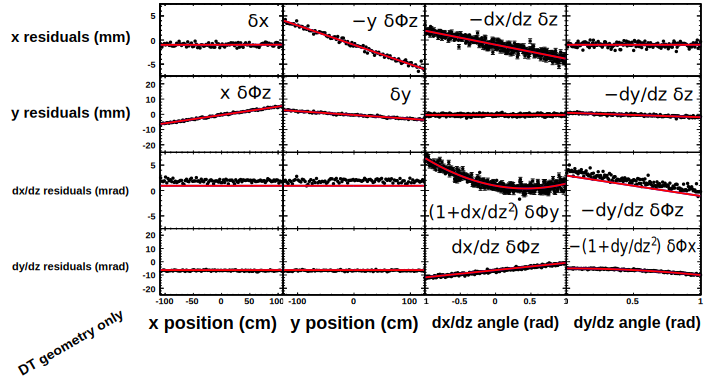
\includegraphics[width=\linewidth]{geometryonly_dt.pdf}
\caption{An example of a fit to 6 misalignment degrees of freedom in a
  ``pure geometry'' DT simulation with only small Gaussian measurement
  errors.  Points are profile histograms of the four residuals versus
  the four track parameters.  Lines are restrictions of the fit
  function with all parameters set to zero except the one shown.  The
  $\Delta \frac{dx}{dz}$ profiles differ from their fit lines because
  the mean of the distribution does not exactly describe its value at
  zero.  Annotations hilight the most significant contribution to each
  plot. \label{fig:geometryonly_dt}}
\end{figure}

\begin{figure}
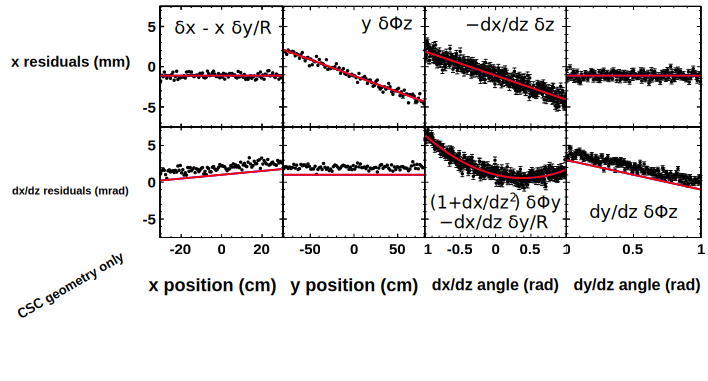
\includegraphics[width=\linewidth]{geometryonly_csc.pdf}

\vspace{-1.5 cm}
\caption{A ``pure geometry'' CSC simulation; see the caption of
  Fig~\ref{fig:geometryonly_dt} for details. \label{fig:geometryonly_csc}}
\end{figure}

\subsection{Fitting the residuals distribution}
\label{sec:fitting}

In the real detector, measurement error contributions to the residuals
are much larger than the systematic distortions we seek to correct.
It is therefore necessary to have a realistic description of the shape
of the measurement error's distribution, so that we can extract
alignment corrections from a global fit to all the parameters that
influence residuals on a chamber.  The measurement effects are:
\begin{itemize}
\item statistical error from the track-fit, amplified by the long
  propagation from Reference to Target (Gaussian),
\item multiple-scattering in material (Gaussian),
\item single-scattering in material (a bell curve with power-law
  tails, see Fig~\ref{fig:residuals_barrel}), and

\begin{figure}
\begin{center} \includegraphics[width=0.4\linewidth]{residuals_barrel.pdf} \end{center}
\caption{Histogram of residuals in log scale to highlight power-law
  tails.  Low-momentum muons are more likely to scatter; hence
  applying a $p_T$ cut varies the tails more than the central Gaussin. \label{fig:residuals_barrel}}
\end{figure}

\item detector resolution (Gaussian and much smaller than the above).
\end{itemize}
The exact power of the single-scattering tail shape, including any
asymmetries it might have, is not significant to the fitted value of
the peak because the Gaussian errors dominate.  We choose to describe
the single-scattering with a Cauchy-Lorentz distribution.  To model
all of the effects, we use a convolution of the two distributions,
\begin{equation}
f(x; x_0, \sigma, \gamma) = \int_{-\infty}^\infty
\frac{1}{\pi}\frac{\gamma}{(x - \xi - x_0)^2 + (\gamma)^2} \times 
\frac{1}{\sqrt{2\pi} \sigma} \exp\left(\frac{-\xi^2}{2
  \sigma^2}\right) \, d\xi \mbox{,}
\label{eqn:fitfunction}
\end{equation}
also known as a Voigt distribution (Fig~\ref{fig:fitfunction}).  We
will describe how this function is applied to residuals momentarily.

\begin{figure}
\begin{center} \includegraphics[width=0.4\linewidth]{fitfunction.pdf} \end{center}
\caption{Fit function for residuals with a Gaussian core and power-law tails.  The residuals in this plot were selected from a geographically small region of the detector (within DT~station~4, wheel~0) to avoid smearing from misalignment. \label{fig:fitfunction}}
\end{figure}

Another important effect is the correlation between $\Delta x$ and
$\Delta \frac{dx}{dz}$ and the correlation between $\Delta y$ and
$\Delta \frac{dy}{dz}$.  Position and angular residuals are correlated
because an angular error early in a track's propagation causes it to
accumulate position error, as presented in
Fig~\ref{fig:sawtooth_diagram}.  The correlation is strongest at the
furthest point from the Reference volume or scattering volume which
introduced the error.

\begin{figure}
\begin{center} 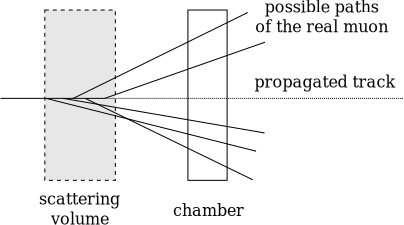
\includegraphics[height=4.5 cm]{sawtooth_diagram.pdf} \end{center}
\caption{Correlation between position residual and angular residual. \label{fig:sawtooth_diagram}}
\end{figure}

A chamber with four residuals components is fitted to the following
four functions simultaneously:
\begin{multline}
f_{\Delta x}\bigg(\Delta x, \, \Delta \tfrac{dx}{dz}, \, x, \, \tfrac{dx}{dz}, \, y, \, \tfrac{dy}{dz}; \, \delta_x, \, \delta_y, \, \delta_z, \, \delta_{\phi_x}, \, \delta_{\phi_y}, \, \delta_{\phi_z}, \, \sigma_{\Delta x}, \, \gamma_{\Delta x}, \, \alpha_{\Delta x} \bigg) = \\
f\bigg(\Delta x; {\Delta x}^{\mbox{\scriptsize geom}}\left(x, \, \tfrac{dx}{dz}, \, y, \, \tfrac{dy}{dz}, \, \delta_x, \, \delta_y, \, \delta_z, \, \delta_{\phi_x}, \, \delta_{\phi_y}, \, \delta_{\phi_z}\right) + \alpha_{\Delta x} \Delta \tfrac{dx}{dz}, \, \sigma_{\Delta x}, \, \gamma_{\Delta x}\bigg)
\label{eqn:fitfunction_x}
\end{multline}
\begin{multline}
f_{\Delta \tfrac{dx}{dz}}\bigg(\Delta \tfrac{dx}{dz}, \, x, \, \tfrac{dx}{dz}, \, y, \, \tfrac{dy}{dz}; \, \delta_x, \, \delta_y, \, \delta_z, \, \delta_{\phi_x}, \, \delta_{\phi_y}, \, \delta_{\phi_z}, \, \sigma_{\Delta \tfrac{dx}{dz}}, \, \gamma_{\Delta \tfrac{dx}{dz}} \bigg) = \\
f\bigg(\Delta \tfrac{dx}{dz}; {\Delta \tfrac{dx}{dz}}^{\mbox{\scriptsize geom}}\left(x, \, \tfrac{dx}{dz}, \, y, \, \tfrac{dy}{dz}, \, \delta_x, \, \delta_y, \, \delta_z, \, \delta_{\phi_x}, \, \delta_{\phi_y}, \, \delta_{\phi_z}\right), \, \sigma_{\Delta \tfrac{dx}{dz}}, \, \gamma_{\Delta \tfrac{dx}{dz}}\bigg)
\label{eqn:fitfunction_dxdz}
\end{multline}
\begin{multline}
f_{\Delta y}\bigg(\Delta y, \, \Delta \tfrac{dy}{dz}, \, x, \, \tfrac{dx}{dz}, \, y, \, \tfrac{dy}{dz}; \, \delta_x, \, \delta_y, \, \delta_z, \, \delta_{\phi_x}, \, \delta_{\phi_y}, \, \delta_{\phi_z}, \, \sigma_{\Delta y}, \, \gamma_{\Delta y}, \, \alpha_{\Delta y} \bigg) = \\
f\bigg(\Delta y; {\Delta y}^{\mbox{\scriptsize geom}}\left(x, \, \tfrac{dx}{dz}, \, y, \, \tfrac{dy}{dz}, \, \delta_x, \, \delta_y, \, \delta_z, \, \delta_{\phi_x}, \, \delta_{\phi_y}, \, \delta_{\phi_z}\right) + \alpha_{\Delta y} \Delta \tfrac{dy}{dz}, \, \sigma_{\Delta y}, \, \gamma_{\Delta y}\bigg)
\label{eqn:fitfunction_y}
\end{multline}
\begin{multline}
f_{\Delta \tfrac{dy}{dz}}\bigg(\Delta \tfrac{dy}{dz}, \, x, \, \tfrac{dx}{dz}, \, y, \, \tfrac{dy}{dz}; \, \delta_x, \, \delta_y, \, \delta_z, \, \delta_{\phi_x}, \, \delta_{\phi_y}, \, \delta_{\phi_z}, \, \sigma_{\Delta \tfrac{dy}{dz}}, \, \gamma_{\Delta \tfrac{dy}{dz}} \bigg) = \\
f\bigg(\Delta \tfrac{dy}{dz}; {\Delta \tfrac{dy}{dz}}^{\mbox{\scriptsize geom}}\left(x, \, \tfrac{dx}{dz}, \, y, \, \tfrac{dy}{dz}, \, \delta_x, \, \delta_y, \, \delta_z, \, \delta_{\phi_x}, \, \delta_{\phi_y}, \, \delta_{\phi_z}\right), \, \sigma_{\Delta \tfrac{dy}{dz}}, \, \gamma_{\Delta \tfrac{dy}{dz}}\bigg)
\label{eqn:fitfunction_dydz}
\end{multline}
That is, the residuals are fitted to four Voigt distributions whose
peak value is the geometric residuals.  The geometric residuals depend
on track parameters $x$, $y$, $\frac{dx}{dz}$, $\frac{dy}{dz}$ and the
6 alignment parameters through
Eqns~\ref{eqn:dtmatrix}--\ref{eqn:cscmatrix}.  The position-residual
distributions include a parameterized offset proportional to its
corresponding angular residual, a skew factor which allows the Voigt
error ellipse to tilt an angle $\tan^{-1}(\alpha)$ in $(\Delta x,
\Delta \frac{dx}{dz})$ space without changing the normalization of the
function.  The product of the four
functions~\ref{eqn:fitfunction_x}--\ref{eqn:fitfunction_dydz}
expresses the likelihood of a $(\Delta x, \Delta \frac{dx}{dz}, \Delta
y, \frac{dy}{dz})$ super-residual as a function of the parameters,
including the 6 alignment parameters.  We perform a weighted, unbinned
maximum liklihood fit for all of the parameters with
MINUIT~\cite{minuit}.  The weights are the
$\left(\chi^2/\mbox{ndf}\right)^{-1}$ of the super-residuals, with the
smallest 1\% of $\chi^2/\mbox{ndf}$ values excluded to avoid spikes in
the distribution.

Though it may seem procedurally complicated, this is functionally a
minimal modification of the HIP procedure used to align the
tracker~\cite{trackerhip}.  In the tracker's HIP procedure, the peak
of the residuals distribution is determined by a weighted mean, which
is equal to a weighted, unbinned maximum likelihood fit to a Gaussian.
The difference in our case is that we allow for long tails in the
distribution due to single-scattering.  The long tails in the fit
function reduce the contribution of outliers to the likelihood
calculation, and thus reduce the influence they have over the peak
position.  (This is why it is necessary to include tails even though
the exact shape is not important.)

The fit is performed in a high-dimensional space with many parameters,
which mandates caution.  It is important to visually inspect the fit
results, a topic which is raised in
section~\ref{sec:validating_residuals_fits} on validating the fit
results.

\subsection{Accomodating errors in magnetic field and material budget}
\label{sec:bfield_errors}

Early in commissioning, track propagation through CMS may suffer from
poor knowledge of the magnetic field map and material budget.  This
would result in incorrect residuals and potentially a wrong alignment.
Since alignment is itself a commissioning task, it must be made
independent of any propagation errors.  Magnetic field and $dE/dx$
errors from an incorrect material budget can be identified by their
distinctive dependencies on momentum, and can both be cancelled by
taking advantage of the fact that they affect residuals in a
charge-antisymmetric way.

\begin{figure}
\subfigure[Diagram for derivation: $x$ is the displacement between straight and helical propagation of a track with radius of curvature $R$ at a distance $\ell$ from the interaction point.  If the field is mis-modelled, it would contribute ${\Delta x}^{\mbox{\scriptsize mag}} = x_{\mbox{\scriptsize track}} - x_{\mbox{\scriptsize muon}}$ to the residual, the difference of two helical propagations with different radii.]{\begin{minipage}{0.45\linewidth} \includegraphics{bfield_diagram.pdf} \vspace{0.5 cm} \end{minipage}} \hfill \subfigure[Derivation of residuals dependence on $q/p_T$ if the magnetic field is mis-modelled.  If the $B_z$ error is also non-uniform, the above holds with ``$\Delta B_z$'' being a (non-trivial) quantity derived from field error along the track's path.]{\begin{minipage}{0.45\linewidth}
\vspace{0.7 cm}
Displacement from straight propagation:
\begin{eqnarray*}
x &=& R \left(1 - \cos\left(\sin^{-1}\left(\ell/R\right)\right)\right) \\
x &\approx& R \left(\frac{1}{2} \left(\ell/R\right)^2\right) = \frac{\ell^2}{2 R} \\
\end{eqnarray*}

\vspace{-0.2 cm}
Relationship to magnetic field $B_z$:
\[ R = \frac{\ell^2}{2 x} = \mbox{300 cm T/GeV } \frac{p_T}{q B_z} \]

Residuals from field error $\Delta B_z$:

\[ \hspace{-1 cm}{\Delta x}^{\mbox{\scriptsize mag}} = \frac{\ell^2}{2 \cdot \mbox{300 cm T/GeV}} \, \left(\frac{q}{p_T}\right) \, \Delta B_z\hspace{-1 cm} \]

\vspace{0.1 cm}
\end{minipage}}
\caption{If the $z$ component of the magnetic field is poorly understood at the time of alignment, the error it contributes to residuals would be proportional to $q/p_T$. \label{fig:bfield}}
\end{figure}

Fig~\ref{fig:bfield} derives the effect of $B_z$ (axial) errors on
$\Delta x$ residuals, which is proportional to $q/p_T$ but not a
simple function of the actual $\Delta B_z$ error.  A similar
derivation would reveal that residuals from $B_r$ (radial) errors are
proportional to $q/p_z$ (Fig~\ref{fig:bfield_components}).
Fig~\ref{fig:superresid_bfield} derives the effect of $B_z$ errors on
$\Delta \frac{dx}{dz}$ residuals, which has a simpler dependence on
magnetic field error, and could even be used to measure corrections to
the field map.

\begin{figure}
\begin{center}
\begin{tabular}{p{0.3\linewidth} c p{0.65\linewidth}}
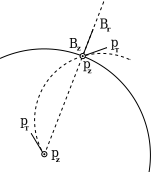
\includegraphics[width=\linewidth]{bfield_components.pdf} & \hspace{0.5 cm} &
\begin{minipage}{\linewidth}
\vspace{-4.5 cm}
\noindent Components affecting $r\phi$ and $\phi_y$ residuals:
\begin{itemize}
\item $|\vec{p}_T \times \vec{B}_z| = |\vec{p}_T| \, |\vec{B}_z|$, always normal to trajectory
\item $|\vec{p}_z \times \vec{B}_r| = |\vec{p}_z| \, |\vec{B}_r|$, approximately normal to trajectory at high momentum
\end{itemize}

\vspace{0.3 cm}
\noindent Components affecting $z$ and $\phi_x$ residuals:
\begin{itemize}
\item $p_T \times B_r$, negligible at high momentum
\end{itemize}

\end{minipage} \\
\end{tabular}
\end{center}
\caption{A summary of magnetic field components which affect residuals. \label{fig:bfield_components}}
\end{figure}

\begin{figure}
\subfigure[Track angles are deflected $\phi = \sin^{-1} \ell/R \approx \ell/R$ relative to a straight-line propagation.  If the magnetic field is mis-modelled, it would add \mbox{$\Delta \phi = \phi_{\mbox{\scriptsize track}} - \phi_{\mbox{\scriptsize muon}}$} to the $\Delta \frac{dx}{dz}$ residual.]{\begin{minipage}{0.45\linewidth} 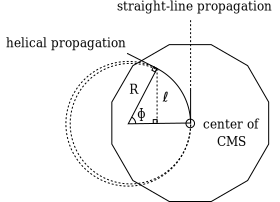
\includegraphics{bfieldangle_diagram.pdf} \vspace{0.2 cm} \end{minipage}} \hfill \subfigure[Derivation of magnetic field contribution to $\Delta \frac{dx}{dz}$ residuals from mis-modelled $B_z$.  If non-uniform, ``$\Delta B_z$'' is a simple average of magnetic field error along the track's path.]{\begin{minipage}{0.45\linewidth}
\vspace{1.75 cm}
\begin{eqnarray*}
R = \frac{\ell}{\phi} &=& \mbox{300 cm T/GeV } \frac{p_T}{q B_z} \\
{\Delta \tfrac{dx}{dz}}^{\mbox{\scriptsize mag}} = \Delta \phi &=& \frac{\ell}{\mbox{300 cm T/GeV}} \left(\frac{q}{p_T}\right) \Delta B_z
\end{eqnarray*}

\vspace{1.75 cm}
\end{minipage}}
\caption{Magnetic field errors would also affect $\Delta
  \frac{dx}{dz}$ residuals, but in a simpler way.  \label{fig:superresid_bfield}}
\end{figure}

Residuals from $dE/dx$ errors have a different momentum dependence,
but the same dependence on charge.  In the momentum range of interest,
the energy muons lose in material is independent of momentum: about
2~MeV~cm$^2$/g, or 1.6~GeV/m through iron.  The track propagator
accounts for known material, so only errors in the material budget
contribute to residuals.  The errors may be positive or negative,
depending on whether the material is overestimated or underestimated.
Re-using the derivations in Figs~\ref{fig:bfield} and
\ref{fig:superresid_bfield}, a constant correction to momentum $p_T \to
(p_T - \Delta)$ yields a correction to $\Delta x$ and $\Delta
\frac{dx}{dz}$ residuals which is proportional to
\begin{equation}
q B_z \left(\frac{1}{p_T} - \frac{1}{p_T - \Delta}\right) \mbox{.}
\end{equation}
Thus the scaling of the effect is inversely quadratic in momentum,
rather than inversely linear:
\begin{equation}
\frac{\frac{1}{p_1} - \frac{1}{p_1 - \Delta}}{\frac{1}{p_2} - \frac{1}{p_2 - \Delta}}
% = \frac{p_2}{p_1} \, \frac{\left(1 - \frac{1}{1 - \Delta/p_1}\right)}{\left(1 - \Delta/p_2\right)}
= \frac{p_2}{p_1} \, \frac{1 - \left(1 - \frac{\Delta}{p_1}\right)^{-1}}{1 - \left(1 - \frac{\Delta}{p_2}\right)^{-1}}
\approx \frac{p_2}{p_1} \, \frac{1 - \left(1 + \frac{\Delta}{p_1}\right)}{1 - \left(1 + \frac{\Delta}{p_2}\right)}
= \left(\frac{p_2}{p_1}\right)^2
\end{equation}

In principle, we could determine all the alignment corrections,
magnetic field errors, and $dE/dx$ errors at once by adding dimensions
and parameters to the fit function.  However, that would unnecessarily
reduce the statistical precision of our alignment measurement.
Instead, we note that both types of propagation errors are
antisymmetric with charge: positive and negative tracks would be
deflected in opposite directions (opposite sign in the residuals
contribution) by either effect (Fig~\ref{fig:antisymmetric_bfield}).

\begin{figure}
\mbox{ } \hfill \subfigure[Both $\vec{B}$ and $dE/dx$ errors affect postive and negative muons in opposite ways.]{\begin{minipage}{4 cm} \vspace{-4 cm} \mbox{ } \hfill 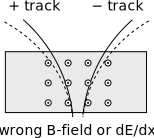
\includegraphics[width=3.5 cm]{antisymmetric_bfield.pdf} \hfill \mbox{ } \end{minipage} \label{fig:antisymmetric_bfield}}
\hfill \subfigure[The two effects depend on momentum, but are still antisymmetric for charges in a given momentum bin.]{\includegraphics[width=4 cm]{demo_residual.pdf} \label{fig:demo_residual}}
\hfill \subfigure[The momentum spectra for the two charges are proportional (cosmic rays shown above).]{\includegraphics[width=4 cm]{demo_momentum.pdf} \label{fig:demo_momentum}} \hfill \mbox{ }
% \mbox{ } \hfill \begin{minipage}{3.5 cm}\vspace{-5.3 cm}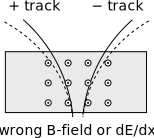
\includegraphics[width=\linewidth]{antisymmetric_bfield.pdf} \end{minipage} \hfill \hfill \includegraphics[height=5.5 cm]{demo_momentum.pdf} \hfill \includegraphics[height=5.5 cm]{demo_residual.pdf} \hfill \mbox{ }
\caption{The two-bin method for cancelling $\vec{B}$ and $dE/dx$ errors: compute corrections separately for positive muons and negative muons, then average the two results. \label{fig:twobin_method}}
\end{figure}

We account for magnetic field and $dE/dx$ errors by computing
alignment corrections separately in two bins, one filled with only
$\mu^+$ and the other filled with only $\mu^-$.  Residuals are biased
by the $\vec{B}$ and $dE/dx$ errors as a function of momentum
(Fig~\ref{fig:demo_residual}), but since $\mu^+$ and $\mu^-$ have
similar spectra in cosmic rays and collisions
(Fig~\ref{fig:demo_momentum}), the biases integrate to equal and opposite
values in the two bins.  The fitted alignment corrections, $\delta_+$
and $\delta_-$, are biased in equal and opposite ways, so we can
compute unbiased corrections by averaging them:
\begin{equation}
\mbox{final alignment corrections} = \frac{\delta_+ + \delta_-}{2} \mbox{.}
\end{equation}
Moreover, we can trace the size of the correction, an overestimate of
the systematic error, by monitoring the difference of the two:
\begin{equation}
\mbox{error tracer} = \frac{\delta_+ - \delta_-}{2} \mbox{.}
\end{equation}
We call this the ``two-bin'' method for cancelling $\vec{B}$ and
$dE/dx$ errors.  It effectively scales up the least populated charge
bin to cancel errors with the other charge bin.

An important caveat is that $\delta_z$ corrections require $\Delta x$
residuals with opposite $\frac{dx}{dz}$ entrance angles to have
opposite signs (see Eqn~\ref{eqn:dtmatrix}).  Charge is highly
correlated with $\frac{dx}{dz}$ entrance angle for geometric reasons,
so this method is unable to correct for biases in $\delta_z$ (see
Fig~\ref{fig:explanation_of_z}).

\begin{figure}
\begin{center}
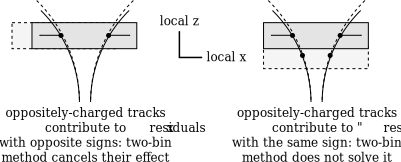
\includegraphics{explanation_of_z.pdf}
\end{center}
\caption{Why the two-bin method cannot correct for bias in $\delta_z$.  \label{fig:explanation_of_z}}
\end{figure}

Positive and negative cosmic rays are known to have proportional
spectra in our momentum range of interest: the charge ratio of cosmic
secondaries is flat as a function of momentum.  Most collisions muons
also have this property, as $b$ and $\bar{b}$ are produced in
equal abundance.  Muons from $W$ bosons may be asymmetric because
$W^+$ and $W^-$ are produced with different rates in $pp$ colliders,
but they are subdominant to $b$/$\bar{b}$.

Fig~\ref{fig:twobin_robust} demonstrates the robustness of the
two-bin method in cosmic rays: a correction in the magnetic field map
adjusts error tracer values, but not alignment residuals from the
averaging technique.

\begin{figure}
\mbox{ } \hfill \includegraphics[height=7 cm]{robustness_alignment1.pdf} \hfill
\includegraphics[height=7 cm]{robustness_errortracer2.pdf} \hfill \mbox{ }
\caption{Alignment residuals and the error tracer before and after a correction to the magnetic field map (in DT~station~4 with cosmic rays).  The alignment residuals are unaffected by the large change in magnetic field values (20--30\%). \label{fig:twobin_robust}}
\end{figure}

\section{Monitoring Tools and Validation/Verification}

Visual monitoring of the alignment procedure is useful for two
purposes: validation and verification.  By ``validation,'' we mean
simply checking that the procedure is valid, that it centers residuals
distributions as intended.  We will reserve the word ``verification''
for measurements that independently determine whether the aligned
chamber positions accord with reality.

A generic example of validation would be to simply run the alignment
procedure twice with the same tracks: if the second alignment yields
zero corrections, then it validates the first alignment.  One way to
actually verify the aligned positions would be to select three
tracking volumes, $A$, $B$, and $C$, where $A$ is used as a reference
to align $B$ and $C$, then $B$ is used as a reference to align $C$
with a different distribution of tracks.  If the two procedures agree
about the position of $C$, then $C$'s result has been independently
verified as a real position in space.

Verification procedures do not need to be completely independent to be
useful.  As long as they contain some new information that is
systematically distinct from the alignment procedure itself, they can
add confidence to the measurement.  Monitorable quantities range from
pure validation to pure verification, and it will be important to keep
in mind roughly how much new information each observable is giving us.

This section will focus on monitoring methods and show example plots,
created under different circumstances, not necessarily the final
alignment.  For summary plots of alignment results, see
sections~\ref{sec:mcstudy} and \ref{sec:craft}.  We only show a
representative subsample of the detailed plots (which are by necessity
numerous), while the summary plots contain the complete results.

\subsection{Validating residuals fits}
\label{sec:validating_residuals_fits}

The alignment fits are performed in a high-dimensional space with many
parameters, which is in principle dangerous.  The fitter has a large
space in which to find an unphysical minimum, and multi-dimensional
data are hard to visualize quantitatively.  Fortunately, our fit
function has a shape that can be easily unfolded and plotted on a 2-D
page.  The fit function is a bell curve (Eqn~\ref{eqn:fitfunction})
with the peak ($x_0$) being a multi-linear function of many variables.
The multi-linear part can be regarded as a set of corrections to the
peak position, which follows a line in parameter space, like the crest
of a mountain ridge.

Fig~\ref{fig:mcfit_extreme_corner2} shows an example of residuals
projections in Monte Carlo.  The example was chosen as an extreme
case, wheel~$\pm$2, station~1, where curves are least Gaussian.
Projections have all of the linear corrections applied to the peak
residuals except for the constant offset, so that the fitted widths,
$\sigma$ and $\gamma$, will be relevant.

\begin{figure}
\includegraphics[height=\linewidth, angle=90]{mcfit_extreme_corner2.pdf}
\caption{An alignment fit in Monte Carlo.  Projections of the four
  residuals are presented along with a scatter plot showing the
  correlation between position and angular residuals.  The red lines
  are fits to the $\mu^+$ residuals (shown) and blue lines are fits to
  the $\mu^-$ residuals (not shown).  The straight lines on the
  scatter plot indicate the correlation slope
  $\alpha$.  \label{fig:mcfit_extreme_corner2}}
\end{figure}

To study the corrections themselves, we plot each of the four
residuals ($\Delta x$, $\Delta \frac{dx}{dz}$, $\Delta y$, and $\Delta
\frac{dy}{dz}$) as a function of each of the four track parameters
($x$, $\frac{dx}{dz}$, $y$, and $\frac{dy}{dz}$).
Fig~\ref{fig:mcfit_misal_and_nongeom} presents an example from
misaligned Monte Carlo with the most important alignment corrections
affecting each plot written on the plots.  The example includes an
``echo,'' a misalignment trend from one distribution appearing in a
different plot because of a correlation between track parameters, in
this case between $x$ and $\frac{dx}{dz}$.  The correlation between
these parameters is expected and illustrated in
Fig~\ref{fig:trackangle_correlation}.  It also includes structure in
$\Delta y$ versus $y$, an effect not accounted for in the track
reconstruction.  After alignment
(Fig~\ref{fig:mcfit_misal_and_nongeom_aligned}), the echo is
eliminated but the structure is not, because the structure is
unrelated to any rigid body parameters.

\begin{figure}
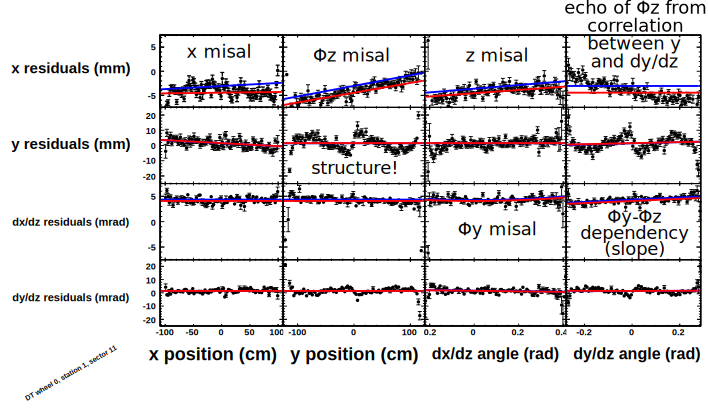
\includegraphics[width=\linewidth]{mcfit_misal_and_nongeom.pdf}
\caption{An annotated example of an alignment fit in Monte Carlo.
  Points are profile histograms of the four residuals versus the four
  track parameters.  Lines are restrictions of the fit function with
  all parameters set to zero except the one shown.  Red corresponds to
  the $\mu^+$ fit and blue to the $\mu^-$
  fit. \label{fig:mcfit_misal_and_nongeom}}
\end{figure}

\begin{figure}
\begin{center}
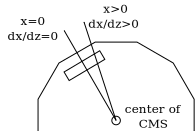
\includegraphics{trackangle_correlation.pdf}
\end{center}
\caption{Expected correlation between $x$ track intersections and
  $\frac{dx}{dz}$ entrance angles. \label{fig:trackangle_correlation}}
\end{figure}

\begin{figure}
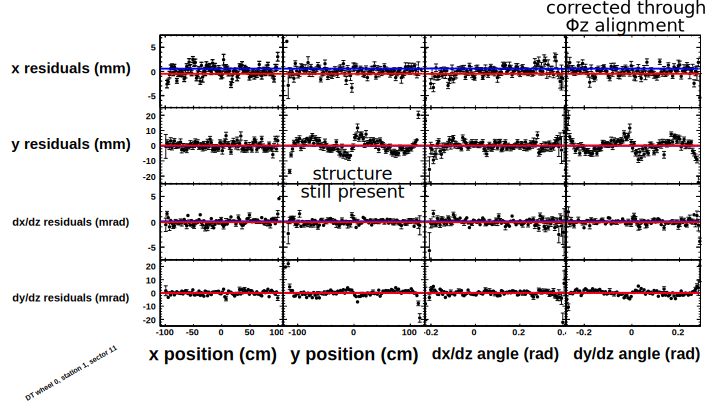
\includegraphics[width=\linewidth]{mcfit_misal_and_nongeom_aligned.pdf}
\caption{The same chamber as Fig~\ref{fig:mcfit_misal_and_nongeom}
  after alignment.  ``Echos'' have disappeared because they are due to
  real alignment corrections in another parameter, but internal DT
  structure is irreducible with rigid body
  parameters. \label{fig:mcfit_misal_and_nongeom_aligned}}
\end{figure}

\subsection{Comparison of geometries in the database}

%% Our first validation tool merely checks to see if geometry
%% descriptions in the conditions database differ, and by how much.  It
%% is actually a program which converts database records into
%% human-readable XML files and a library for plotting geometrically
%% relevant differences in pyROOT.  The conversion can be reversed: the
%% same XML descriptions can be uploaded to the database as muon
%% alignments for track-reconstruction.  The features of this system are
%% all documented on its own twiki page:
%% SWGuideMuonGeometryConversion~\cite{SWGuideMuonGeometryConversion}.

%% In this note, we use the conversion tool to prepare test-pattern and
%% randomized misalignment scenarios for the Monte Carlo study, and to
%% plot differences in chamber parameters with respect to ideal.

\subsection{Muon system maps}

The fit-validation plots presented trends in residuals distributions
inside each chamber.  These trends were expected because they are
caused by misalignments.  However, if there are unexpected biases in
the tracks used for alignment, either due to tracker misalignments or
propagation errors, they would show up as trends in the residuals that
cross chamber boundaries.  To verify our expectation that residuals
are correlated within each chamber and uncorrelated outside, we plot
maps of the residuals across the whole muon system.

The measurement planes of the DT chambers lie nearly flat in $\phi$
and $z$, so these are the relevant abscissas for the map plots.  To
make sure that no more than one chamber corresponds to each bin in the
plots, the plots versus $z$ must be split by sector, the plots versus
$\phi$ must be split by wheel, and all plots must be split by station.
The endcaps have 18 rings which are one CSC thick (counting ME1/1a as
being distinct from ME1/1b), so each of these gets a separate $\phi$
plot.  The CSCs lie flat in $\phi$ and the radial direction, instead
of $z$, so the orthogonal plots are 36 radial spokes for each of the 8
disks.  Some examples are shown in Fig~\ref{fig:examplemap_rphi}.

\begin{figure}
\hspace{0.5 cm} \includegraphics[height=0.8\linewidth, angle=90]{examplemap_rphi1.pdf}

\hfill \includegraphics[height=0.8\linewidth, angle=90]{examplemap_rphi4.pdf} \hspace{0.5 cm}

\hspace{0.5 cm} \includegraphics[height=0.8\linewidth, angle=90]{examplemap_CSCrphi1.pdf}

\caption{Three maps of residuals before and after alignment in Monte Carlo: DT station 1, wheel 0 (top), station 4 wheel $+$2 (middle), and CSC ME$+$1, chamber 18 (bottom).  Chamber identities were not used to make the plots; boundaries are overlaid on the results. \label{fig:examplemap_rphi}}
\end{figure}

On each of these axes, we plot all 6 alignment results: $\delta_x$,
$\delta_y$, $\delta_z$, $\phi_x$, $\phi_y$, and $\phi_z$, as well as
the antisymmetric combination of fit results to trace
$\vec{B}(\vec{x})$ and $dE/dx$ errors.  Every bin is derived from the
full fitting procedure described in
% section~\ref{sec:alignment_from_fits}, though parameters equivalent to  % nope
section, though parameters equivalent to  % nope
the binning are fixed.  (Letting the slope of residuals versus $x$
float in a dataset representing a narrow slice in $x$ would
statistically weaken all of the fit's results.)  As with the
fit-validation, there are too many plots to publish, but they are
useful for diagnostics.  An example of DT $\delta_z$ (radial
displacement) in cosmic ray data is presented in
Fig~\ref{fig:examplemap_zpos}.  This is a complicated quantity, the
slope of fits to residuals versus track entrance angle, and it shows
clear discontinuities at the chamber boundaries, indicating a real
misalignment.

\begin{figure}
\includegraphics[height=\linewidth, angle=90]{examplemap_DATAzpos.pdf}
\caption{Results of $\delta_z$ fits (radial alignment for DT chambers) as a function of global $z$ position.  Results agree within each chamber and disagree with their neighbors, indicating real radial misalignments. \label{fig:examplemap_zpos}}
\end{figure}

The muon system maps are the basis for binned-residual summary plots,
where the points in the maps are used to fill a histogram, and
therefore present all of the data on one page (trading depth for
breadth).  Such a plot is more incisive than a simple histogram of
residuals, because pre-averaging the residuals in geographically
relevant bins highlights systematic deviations from zero, rather than
hiding it under track-by-track scattering.  The width of the
binned-residual distribution depends on the size of the bins, but they
are standardized: 180 bins in $\phi$ from $-\pi$ to $\pi$, 60 bins in
$z$ from $-660$~cm to $660$~cm (for DTs), and 60 bins in radial
position, from $100$~cm to $700$~cm (for CSCs).
Fig~\ref{fig:twobin_robust} from section~\ref{sec:bfield_errors}
presented histograms of residuals binned in $z$.

\subsection{Verification with relative residuals}

The map plots provide some verification of the alignment in that they
meaningfully compare residuals from the same chamber with residuals
from neighboring chambers, and thus distinguish between distortions
related to the chamber and distortions related to the tracks.
However, they are the same residuals that were used to perform the
alignment, and are therefore not independent.

Independent sets of residuals allow us to more fully verify the
alignment by triangulation: after having aligned each chamber
individually to the tracker, we check the alignment with residuals on
tracks connecting the chambers themselves.  One way to do this re-uses
the alignment tracks, but ignores position information from the
tracker.  Consider the difference of residuals between two stations on
each track, diagrammed in Fig~\ref{fig:residuals_difference}:
\begin{figure}
\begin{center}
\includegraphics[height=7 cm]{residuals_difference.pdf} \hspace{1 cm} \includegraphics[height=7 cm]{residdiff23.pdf}
\end{center}
\caption{Relative residuals are linearly independent from the
  residuals used in alignment, and can therefore verify its
  correctness.  PLACEHOLDER!  This plot is from the old (3-parameter)
  CRAFT alignment.  AND it is the only one that showed (marginal)
  improvement--- stations 1$-$2 and 3$-$4 showed (marginal)
  degradation.  (We interpret the three as indicating no net change in
  {\it relative} positions.)  In the new plot, we will combine all stations, since they have comparable widths. \label{fig:residuals_difference}}
\end{figure}
\begin{multline}
\mbox{residuals difference}(3, 2) = (\mbox{station 3 track impact point} - \mbox{station 3 hit position}) - \\
(\mbox{station 2 track impact point} - \mbox{station 2 hit position})\mbox{.}
\end{multline}
The tracker's position information cancels in the residuals
difference, as well as any random scattering that happens between the
tracker and station~2.  The residuals difference is therefore a
narrower distribution than absolute residuals and represents the
relative alignment of chambers in station~2 and chambers in station~3
(sector by sector).  The advantage unique to this method is that the
track retains momentum magnitude information from the tracker: it is a
curved ruler, where the appropriate curvature is determined by the
tracker's high-precision momentum measurement.  The difference can be
calculated for any pair of neighboring stations, but is difficult to
interpret for DT stations~4 and 3, because the sector boundaries in
station~4 do not line up with those in station~3.

A more extensive version of the same idea uses a set of aligned
chambers as a new reference for track-fitting and re-aligning their
neighbors.  Chambers aligned by both methods verify the technique,
though with less precision because the momentum resolution of the muon
system is not as high as the tracker.  Without collisions, this is the
only way to align some chambers in the muon system, because the
constraint requiring cosmic rays to pass through the tracker yields
very few tracks in the high $|z|$ regions of the detector.

\section{Global alignment results with collisions Monte Carlo}
\label{sec:mcstudy}

A study of alignment with 50~pb$^{-1}$ of simulated muons from QCD
(primarily $b\to\mu$, which is the majority of the muons that we'll
see).  I have the event samples in AlCaReco format, so it's ready to
go.  I've put it on hold until the tracker alignment is sufficiently
well understood for us to do a combined alignment study which will
become the new 50 and 200~pb$^{-1}$ alignment scenarios.

\subsection{Scaling with statistics}

\subsection{Dependence on tracker misalignment}

\subsection{Dependence on magnetic field errors}

\section{Global alignment results with cosmic ray data}
\label{sec:craft}

I've described all of the method and plotting techniques, so this
section will be light on text and heavy on plots with interpretations.
I'm running the alignment now, and re-running it with small changes in
the configuration to optimize our use of the data.  I'll make all of
the plots when I have a final alignment, ready to be used for
tracker-pointing re-processing.

\subsection{Validation plots}

\subsection{Verification with relative residuals}

\subsection{Verification with stand-alone muon alignments}

This will take several weeks longer than everything else.

\subsection{Verification with cosmic track splitting}

Cosmic track splitting study by Nhan Tran and Alessio Bonato applied
to global muons.  It's independent because nothing in the alignment
procedure explicitly correlated the top chambers with the bottom
chambers.  It will need to be repeated with the new alignment (as well
as the new magnetic field, new tracker alignment, and new tracker
weights).  Naturally, they'll need to be acknowledged.

\section{Relative alignment of CSCs with local tracks}

We have focused so far on global alignment because of its importance
in muon track-fitting, but local alignment methods have a different
set of advantages which can be used to improve our overall
understanding.  Locally-propagated tracks, for instance from one
chamber to its neighbor, suffer far less from propagation errors,
yielding narrower residuals distributions and fewer systematic
uncertainties.  High precision can be achieved with fewer tracks
because of the narrowness of the residuals, and the track source need
not point to the tracker, so the endcap can be aligned before first
collisions with beam-halo data.  When collisions muons are available
for the global alignment procedure, local alignment will severely test
it and provide diagnostics in the case of a disagreement.

The disadvantage of local alignment algorithms is that they do not
relate the coordinate frame of the aligned system to a common
standard.  In this section, we will describe a procedure that aligns
CSCs within rings, but does not relate the aligned rings to each other
or the tracker.  Global muons from collisions will be required to make
this connection, though we can combine residuals from all the chambers
in each ring to minimize statistical uncertainty and average over
possible systematic effects.

\subsection{Description of the CSC Overlaps algorithm}
\label{sec:overlaps_algorithm}

In the muon endcap, CSCs were designed to overlap slightly with their
neighbors for the purpose of local alignment.  In each ring except
ME1/3, tracks on the left edge of chamber~$i$ can be expected to also
pass through the right edge of chamber~$i+1$, so both chambers can
independently determine the track parameters with all 6 layers.  If
these chambers systematically disagree about the positions of tracks
in a shared coordinate system, then one or both are misaligned.
Relative alignment corrections can be propagated through the ring
until we return to the first chamber, at which point the collection of
chambers must form a consistent circle, a constraint known as closure.

This can be made more formal by defining $N$ = 18 or 36 alignment
corrections $A_i$ (where $i \in \{1\ldots 18\}$ for ME2/1, ME3/1,
ME4/1 and $i \in \{1\ldots 36\}$ for the other stations).  The ring
also has $N$ residuals distributions, but each residuals distribution
corresponds to a pair of chambers, not an individual chamber, because
each residual is the position of the track as measured in chamber~$i$
minus the position of the track as measured in chamber~$i+1$.  (Index
arithmetic should be presumed to be mod $N$, such that $i+1=1$ when
$i=N$.  Remember that the chambers are arranged in a circle.)  To use
the language of the preceeding sections in this note, we may think of
one chamber as the reference tracking volume and the other as the
target to be aligned, except that there is no reason to prefer one as
a reference above the others.  Label the mean of the residuals
distribution corresponding to chambers~$i$ and $i+1$ as
$\alpha_{i\mbox{\scriptsize, }i+1}$.  We can use the mean of the
residuals distribution, rather than a fit for its peak, because
scattering is not an issue.

If we move chambers~$i$ and $i+1$ by $A_i$ and $A_{i+1}$, the mean of
the overlap residuals can be expected to change from
$\alpha_{i\mbox{\scriptsize, }i+1}$ to
$\alpha_{i\mbox{\scriptsize, }i+1} - (A_i - A_{i+1})$.  We want to find
a complete set of corrections to minimize all of the residuals means,
so we define a $\chi^2$ as
\begin{equation}
\chi^2 = (\alpha_{12} - A_1 + A_2)^2 + (\alpha_{23} - A_2 + A_3)^2 + \ldots + (\alpha_{N1} - A_N + A_1)^2
\end{equation}
and minimize it by setting its derivatives to zero.  For example,
\begin{equation}
\frac{1}{2} \frac{\partial \chi^2}{\partial A_2} = (\alpha_{12} - A_1 + A_2) - (\alpha_{23} - A_2 + A_3) = 0 \mbox{.}
\end{equation}
The complete set of such equations, written in matrix form, looks like
the following (with $N=5$ for brevity):
\begin{equation}
\left(\begin{array}{c}
\alpha_{12} - \alpha_{51} \\
\alpha_{23} - \alpha_{12} \\
\alpha_{34} - \alpha_{23} \\
\alpha_{45} - \alpha_{34} \\
\alpha_{51} - \alpha_{45}
\end{array} \right)
=
\left(\begin{array}{r r r r r}
2 & -1 &  &  & -1 \\
-1 & 2 & -1 &  &  \\
 & -1 & 2 & -1 &  \\
 &  & -1 & 2 & -1 \\
-1 &  &  & -1 & 2
\end{array}\right)
\left(\begin{array}{c}
A_1 \\
A_2 \\
A_3 \\
A_4 \\
A_5 \\
\end{array} \right)\mbox{.}
\label{eqn:NbyNmatrix}
\end{equation}
To align all $N$ chambers, we need only invert this $N\times N$
matrix.  We did not break the symmetry between the reference system
and the target system: this procedure mutually aligns all chambers at
once.

Unfortunately, the matrix in Eqn~\ref{eqn:NbyNmatrix} is singular
because a procedure like this cannot determine the global position of
the whole system.  Adding the same constant to every $A_i$, which
would rotate the whole ring rigidly, would leave the $\chi^2$
invariant because the relative positions of every pair of chambers is
unchanged by the collective motion.  Since there is a direction in
$\{A_i\}$-space in which $\chi^2$ is flat, it cannot be minimized by
setting its derivatives to zero.  One way to solve the problem is to
refuse motion in the flat direction by fixing one chamber, e.g.\ force
$A_1=0$ and make chamber~1 the reference.
\begin{equation}
\left(\begin{array}{c}
0 \\
\alpha_{23} - \alpha_{12} \\
\alpha_{34} - \alpha_{23} \\
\alpha_{45} - \alpha_{34} \\
\alpha_{51} - \alpha_{45}
\end{array} \right)
=
\left(\begin{array}{r r r r r}
1 & 0 & 0 & 0 & 0 \\
-1 & 2 & -1 &  &  \\
 & -1 & 2 & -1 &  \\
 &  & -1 & 2 & -1 \\
-1 &  &  & -1 & 2
\end{array}\right)
\left(\begin{array}{c}
A_1 \\
A_2 \\
A_3 \\
A_4 \\
A_5 \\
\end{array} \right)
\end{equation}
However, if chamber~1 is misaligned, it would take the whole ring with
it.  Ring misalignments can be corrected later with global alignment,
but it is best to avoid introducing them.  Instead, we can make the
flat direction quadratic in $\chi^2$ by preferring $\{A_i\}$ sets that
have an average of zero (minimally rotate the ring).  This can be
accomplished by adding a term like
\begin{equation}
\left[ \frac{1}{N} \left(A_1 + A_2 + \ldots + A_N\right) \right]^2
\label{eqn:average}
\end{equation}
to the $\chi^2$.  Each derivative equation becomes
\begin{equation}
\frac{1}{2} \frac{\partial \chi^2}{\partial A_i} = (\alpha_{i-1\mbox{\scriptsize, }i} - A_{i-1} + A_i) - (\alpha_{i\mbox{\scriptsize, }i+1} - A_i + A_{i+1}) + \frac{1}{N^2} \sum_{i=1}^N A_i = 0 \mbox{,}
\end{equation}
so the matrix equation is now
\begin{equation}
\left(\begin{array}{c}
\alpha_{12} - \alpha_{51} \\
\alpha_{23} - \alpha_{12} \\
\alpha_{34} - \alpha_{23} \\
\alpha_{45} - \alpha_{34} \\
\alpha_{51} - \alpha_{45}
\end{array} \right)
=
\left[\left(\begin{array}{r r r r r}
2 & -1 &  &  & -1 \\
-1 & 2 & -1 &  &  \\
 & -1 & 2 & -1 &  \\
 &  & -1 & 2 & -1 \\
-1 &  &  & -1 & 2
\end{array}\right)
+
\frac{1}{N^2}
\left(\begin{array}{r r r r r}
1 & 1 & 1 & 1 & 1 \\
1 & 1 & 1 & 1 & 1 \\
1 & 1 & 1 & 1 & 1 \\
1 & 1 & 1 & 1 & 1 \\
1 & 1 & 1 & 1 & 1
\end{array}\right)
\right]
\left(\begin{array}{c}
A_1 \\
A_2 \\
A_3 \\
A_4 \\
A_5 \\
\end{array} \right)\mbox{.}
\label{eqn:solution}
\end{equation}
It has a unique solution in which the average correction
(Eqn~\ref{eqn:average}) is minimized to exactly zero.  Actually, adding
any non-zero constant to every element would yield the same solution as
the physically-motivated $\frac{1}{N^2}$.

The circular ring of chambers also provides an internal cross-check:
the sum of the means of pairwise residuals must be zero.  If not, no
combination of alignment corrections can center all of the residuals,
because
\begin{equation}
\mbox{closure} = \sum_{i=1}^N \alpha_{i\mbox{\scriptsize, }i+1} - (A_i - A_{i+1}) = \sum_{i=1}^N \alpha_{i\mbox{\scriptsize, }i+1}
\end{equation}
is independent of $\{A_i\}$.  (Note that $\sum_{i=1}^N A_{i+1}$ is
just a reindexing of $\sum_{i=1}^N A_i$ because index arithmetic is
understood to be mod $N$.)  With non-zero closure, the solution of
Eqn~\ref{eqn:solution} uniformly distributes residuals so that they
all have non-zero means, which is to say, every chamber disagrees with
its neighbor about where the tracks are.  Unclosed $r\phi$ residuals
either imply
\begin{itemize}
\item the average distance of the chambers from the beamline is
  incorrect, or
\item the presumed width of the chambers is incorrect.
\end{itemize}
In the first case, the circumference of the ring is miscalculated
because the wrong radius is assumed; in the second case, the wrong arc
is assumed per chamber.  In the course of developing this technique,
we discovered a 15~mm closure error, which derived from an 800~$\mu$m
error in the active width of the chamber description, ultimately from
a 0.09\% error in the pitch angle of each cathode strip (10~$\mu$m per
strip).  It is a very sensitive technique!

\subsection{Local CSC alignment parameters}

As much as possible, the same techniques are used to calculate
residuals and alignment corrections in the local procedure as in the
global.  Tracks propagated to a chamber are compared with the
chamber's segment position and angle, much like the super-residuals
described in section~\ref{sec:super_residuals}.  Anode wire
measurements are ignored due to their large granularity, and strips
are taken to measure curvilinear $r\phi$ residuals, rather than
cartesian local $x$, again in direct analogy with the global
procedure.  The difference is that the source for global tracks is the
tracker, propagated through magnetic fields and many radiation lengths
of material, while local tracks are extrapolations from a linear fit
in the neighboring chamber.  To treat the pair of chambers
symmetrically, hits in each are fitted to line segments on the surface
of a cylinder around the beamline
\begin{equation}
\phi(z) = a + bz
\end{equation}
and the parameters of these two fits are compared at the plane
equidistant between the chamber centers (at $z = (z_1 + z_2)/2$, where
$z_1$ and $z_2$ are the global $z$ positions of the two chambers).

Three parameters are accessible with this technique (Fig~\ref{fig:overlaps_parameters}):
\begin{enumerate}
\item the relative
$\phi_y$ of the two chambers is their average difference in slopes ($\Delta b$),
\item the relative $\delta_{r\phi}$ position is the difference in intercepts ($\Delta
a$), and
\item the relative $\phi_z$ angle is the difference in intercepts
as a function of hit position ($d(\Delta a)/dy$).  
\end{enumerate}
These parameters are interdependent in the sense that the
$\delta_{r\phi}$ result depends on $\phi_y$ and the $\phi_z$ result
depends on $\delta_{r\phi}$, but the dependencies are unidirectional.
If corrected in the above order, first $\phi_y$, then $\delta_{r\phi}$, then
$\phi_z$, the parameters decouple, avoiding the need for a combined
fit.

\begin{figure}
\subfigure[Determination of $\phi_y$ from slopes.]{\includegraphics[width=0.35\linewidth]{topview_1.pdf}} \hfill \subfigure[Determination of $\delta_{r\phi}$ from intercepts at $z=0$.]{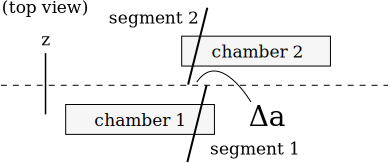
\includegraphics[width=0.35\linewidth]{topview_2.pdf}} \hfill \subfigure[Determination of $\phi_z$ from $d(\Delta a)/dy$.]{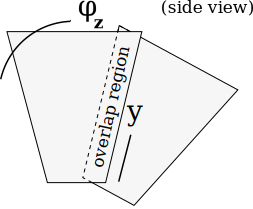
\includegraphics[width=0.2\linewidth]{sideview.pdf}}
\caption{The three alignment parameters accessible to local track matching in CSCs. \label{fig:overlaps_parameters}}
\end{figure}

The formalism developed in section~\ref{sec:overlaps_algorithm}
can be applied to each parameter separately.  First,
$\alpha_{i\mbox{\scriptsize, }i+1}$ is defined as $b_i - b_{i+1}$ and $A_i$
as ${\phi_y}_i$ to align the angles, then
$\alpha_{i\mbox{\scriptsize, }i+1}$ becomes $a_i - a_{i+1}$ and $A_i$
becomes ${\delta_{r\phi}}_i$ to align the positions, and similarly for
$\phi_z$.

\subsection{Specialized trigger and data streams}

Only events with muons that thread the narrow overlaps between
chambers are useful to this procedure, which is a small fraction of
the whole.  Beam-halo and collisions muons are equally useful, but
they come from different sources (primary datasets) because they're
reconstructed differently.  We therefore have special triggers and
data streams for each case, to avoid losing events to generic
prescales.

Four triggers are designed to accept beam-halo events.  They are
\begin{itemize}
\item HLT\_CSCBeamHalo: simply passes L1\_SingleMuBeamHalo bit, likely
  to be prescaled,
\item HLT\_CSCBeamHaloRing2or3: same but additionally requires
  reconstructed hits in ME$n$/2 or ME1/3, which are less common and
  therefore deserve a lower prescale,
\item HLT\_CSCBeamHaloOverlapsRing1 and Ring2: requires clusters of
  reconstructed hits in neighboring chambers, consistent with a muon
  in the overlap region.
\end{itemize}
Naturally, the two specialized overlaps triggers are essential to the
CSC Overlaps procedure; the others are for cross-checks and detector
studies which may be unrelated to alignment.  To produce one complete
ME$n$/1 alignment per day, we would need 0.4~Hz from
HLT\_CSCBeamHaloOverlapsRing1, and for one ME$n$/2 alignment per day,
we would need 0.8~Hz from HLT\_CSCBeamHaloOverlapsRing2 (scaling from
2008 exercise).

Events with beam-halo trigger bits are then collected by the
MuAlBeamHaloOverlaps AlCaReco stream (similar to MuAlCalIsolatedMu,
MuAlGlobalCosmics, and MuAlStandAloneCosmics, discussed on
page~\pageref{page:AlCaReco}).  MuAlBeamHaloOverlaps has no explicit
$p_T$ cut (the momentum of tracks parallel to $\vec{B}$ would not be
measured well anyway), with an option to apply a coarse energy cut by
requiring the reconstructed track to pass through a given number of
stations.

Collisions muons to be used with the CSC Overlaps procedure are
collected with the standard single-muon triggers and whatever
prescales that implies (in flux at the low end of the momentum scale).
They are then delivered to alignment via the MuAlOverlaps stream.  As
usual, the AlCaReco streams contain only what is needed for alignment:
tracks and the hits associated with those tracks, so they use very
little disk space for the number of events they contain.

\subsection{Results from the 2008 LHC run}

On September 10--17, 2008, protons circulated in the LHC tunnel,
providing a source of beam-halo muons which we used to test the CSC
Overlaps procedure.  Three-quarters of the beam-halo events were
collected from a 9-minute run on the evening of September 11 (run
number 60232; 33,000 HLT\_CSCBeamHaloOverlapsRing1 triggers).  To
guarantee a consistent snapshot of the detector geometry, we select
data from this run only.  The CSC Overlaps procedure is only
meaningful when applied to rings in which all chambers are actively
taking data; missing data in any one chamber removes two residuals
constraints (e.g.\ $\alpha_{i-1\mbox{\scriptsize, }i}$ and
$\alpha_{i\mbox{\scriptsize, }i+1}$), making Eqn~\ref{eqn:solution}
unsolvable.  In this run, ME$-$2/1 and ME$-$3/1 were the only
completely-active rings (the beam was coming from the minus side of
CMS, which contributed significantly more muons to the minus endcap).
Many of the CSC commissioning problems experienced in 2008 have been
fixed in the long shut-down, so we can expect more complete rings in
2009.

The procedure was first applied to beam-halo Monte Carlo with
approximately the same number of events but a different azimuthal and
radial distribution than the real beam.  (The azimuthal and radial
distribution of the real beam varied considerably from run to run,
more than the difference between our chosen run and the Monte Carlo.)
Fig~\ref{fig:overlaps_mc} presents the results from a simulated
alignment procedure, starting from a standard misaligned geometry
(2008 ``STARTUP'' scenario).  The standard deviation of the difference
between aligned chamber positions and MC truth quantifies the
precision of the technique, though the interpretation is approximate
because of the differences in track distribution.

\begin{figure}
\subfigure[$\phi_y$ precision is $\sim$1~mrad]{\includegraphics[width=0.3\linewidth]{mcchamber_phiy.pdf}} \hfill \subfigure[$\delta_{r\phi}$ precision is $\sim$230~$\mu$m]{\includegraphics[width=0.3\linewidth]{mcchamber_rphi.pdf}} \hfill \subfigure[$\phi_z$ precision is $\sim$0.25~mrad]{\includegraphics[width=0.3\linewidth]{mcchamber_phiz.pdf}} \hfill
\caption{Comparison of alignment parameters with MC truth before (dark) and after (light) a simulated beam-halo alignment with similar statistics to the 2008 LHC run. \label{fig:overlaps_mc}}
\end{figure}

To verify the aligned positions of chambers in real data, we compare
the beam-halo results with photogrammetry, an alignment derived from a
literal photograph of the detector.  Each chamber has two alignment
pins, connected directly to the active layer planes and capped with a
reflective disk, the center of which is accurately measured by the
photographs.  An average of the two pin positions yields the $r\phi$
location of the chamber and a difference of the two pin positions,
divided by the distance between the pins, yields the $\phi_z$ angle.
The $\phi_y$ angle is inaccessible to photogrammetry, because both
pins lie on the chamber's local $y$ axis.  The photogrammetry results
are clearly independent from the track-based results, and can
therefore be used to verify the latter.  The beam-halo data were
collected with no magnetic field, just like the photogrammetry, so we
can be confident that they describe the same geometry.

Fig~\ref{fig:overlaps_data1} presents the aligned value of each
parameter of each chamber relative to ideal values for both
track-based alignment and photogrammetry.  One can see that the two
methods are both measuring significant differences with respect to
ideal, and that the results are highly correlated.

\begin{figure}
\begin{center}
\hspace{-1.3 cm} \begin{minipage}{1.2\linewidth}
\includegraphics[height=0.45\linewidth, angle=90]{compare_m21_phiy.pdf} \includegraphics[height=0.45\linewidth, angle=90]{compare_m31_phiy.pdf}

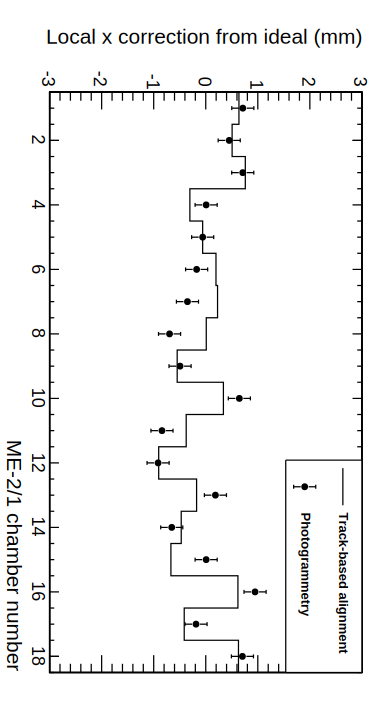
\includegraphics[height=0.45\linewidth, angle=90]{compare_m21_x.pdf} 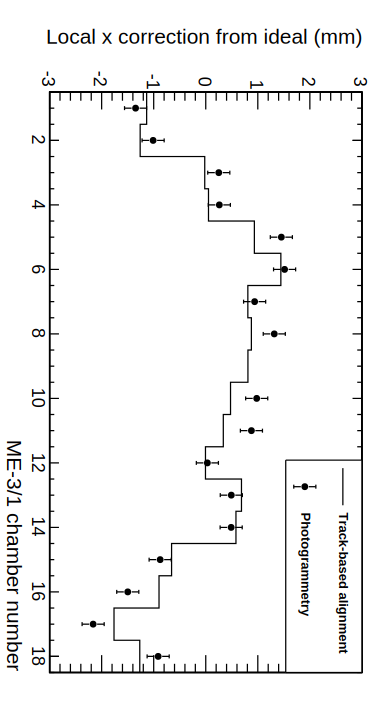
\includegraphics[height=0.45\linewidth, angle=90]{compare_m31_x.pdf}

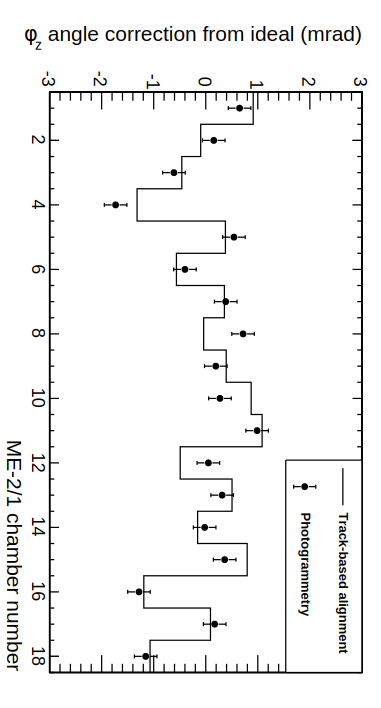
\includegraphics[height=0.45\linewidth, angle=90]{compare_m21_phiz.pdf} 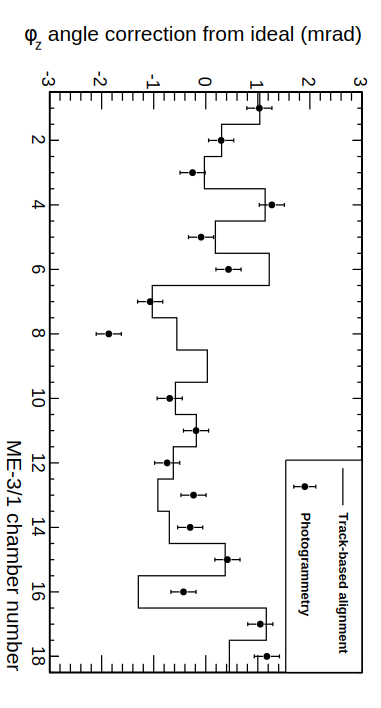
\includegraphics[height=0.45\linewidth, angle=90]{compare_m31_phiz.pdf}
\end{minipage}
\end{center}
\caption{CSC alignment results from the Overlaps procedure and the 2008 LHC run, presented as a difference from ideal and compared with photogrammetry where possible. \label{fig:overlaps_data1}}
\end{figure}

To compute the accuracy of the beam-halo alignment with photogrammetry
as the reference, we subtract the $\delta_{r\phi}$ and $\phi_z$ of
each beam-halo result from the corresponding photogrammetry result
(Fig~\ref{fig:overlaps_data2}).  The mean (bias) is consistent with
zero, but in the $\delta_{r\phi}$ case, a non-zero mean would
correspond to a global rotation of the disk which is not a measurable
parameter in the CSC Overlaps procedure or the single-disk
photogrammetry.  The standard deviations are 340~$\mu$m in
$\delta_{r\phi}$ and 0.42~mrad in $\phi_z$, which derive from a sum in
quadrature of the track-based uncertainties and the photogrammetry
uncertainties.  Photogrammetry uncertainties are 300~$\mu$m for each
pin \cite{photogrammetry}, which means $\mbox{(300~$\mu$m)}/\sqrt{2} = 210$~$\mu$m for
the chamber center position and $\mbox{(300~$\mu$m)} \cdot \sqrt{2} /
\mbox{1.85~m} = 0.23$~mrad for the chamber angle.  Subtracting the
photogrammetry uncertainties in quadrature from standard deviations
observed in the plots,
\begin{eqnarray}
\mbox{track-based $\delta_{r\phi}$ accuracy} &=& \sqrt{(\mbox{340~$\mu$m})^2 - (\mbox{210~$\mu$m})^2} = \mbox{270~$\mu$m} \\
\mbox{track-based $\phi_z$ accuracy} &=& \sqrt{(\mbox{0.42~mrad})^2 - (\mbox{0.23~mrad})^2} = \mbox{0.35~mrad}
\end{eqnarray}

\begin{figure}
\begin{center}
\includegraphics[width=0.45\linewidth]{delta_translations_goodcolors.pdf} \includegraphics[width=0.45\linewidth]{delta_rotations_goodcolors.pdf}
\end{center}
\caption{Chamber-by-chamber verification of the beam-halo alignment with photogrammetry.  The dark histogram is before alignment; the light histogram and statistics box are after alignment. \label{fig:overlaps_data2}}
\end{figure}

Thus, the 200-300~$\mu$m accuracy goals are already demonstrated in a
subset of endcap chambers, using a local alignment technique.  There
is no indication that this result is systematically limited; much
higher precision may be possible once we collect more than 12~minutes
of data.

\subsection{Extension to align CSC layers}
\label{sec:CSC_layer_alignment}

The CSC Overlaps procedure can be extended to align CSC layers, though
the layer procedure only needs to be applied once with high
statistics, rather than routinely with a maintainable algorithm.  The
usual difficulty in aligning layers with local tracks is that the
systems are underconstrained.  Extra constraints applicable to tracks
overlapping well-aligned neighbors allow us to break all of the
important degeneracies.

Local alignment procedures require tracks to be fitted locally, which
introduces an interdependency between track-fitting and alignment.  In
the CSC Overlaps procedure, we needed the circular closure constraint
to form an overconstrained system, and no such thing is available
inside of a chamber.  In a chamber, there are 6 layers; in principle,
5 need to be aligned, since the collective position of all the layers
is a chamber-alignment issue.  But it takes at least 2 parameters to
determine each track: one too many.  If we simply ignore this fact and
constrain the track to two of the layers, we would not know if the
layers are skewed like a deck of cards
(Fig~\ref{fig:layer_alignment_skew}), a plausible misalignemnt, as it
could be caused by a simple tilt of the alignment pins.  Small tilts
could also escape quality control at the production sites, which
measured cathode traces relative to the pins.

\begin{figure}
\begin{center}
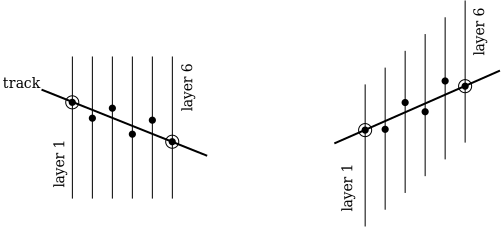
\includegraphics[width=0.75\linewidth]{layer_alignment_skew.pdf}
\end{center}
\caption{Even when a track is constrained to two only layers, the positions of the other layers can only be determined up to a collective offset and a collective skew.  The two situations depicted here are indistinguishable. \label{fig:layer_alignment_skew}}
\end{figure}

A well-aligned pair of neighboring chambers can be treated as a
single, 12-layer chamber for tracks that pass through the overlap
region.  Once misalignments between the two chambers have been
corrected with the CSC Overlaps procedure, we can justifiably assume
that the 12-layer system is not collectively skewed, and align 10 of
the layers to a track constrained to 2 layers (or an equivalent
average that maintains the same number of degrees of freedom).  Such a
procedure is illustrated in Fig~\ref{fig:layer_alignment_noskew}.

\begin{figure}
\begin{center}
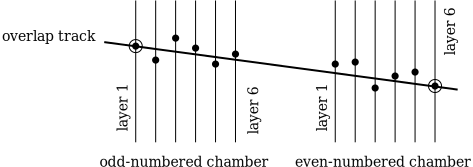
\includegraphics[width=0.75\linewidth]{layer_alignment_noskew.pdf}
\end{center}
\caption{Method for aligning layers within chambers: constrain a linear track to the first and last layers in a two-chamber overlap, then align the remaining layers to that track. \label{fig:layer_alignment_noskew}}
\end{figure}

Using beam-halo data from 2008, we applied the above procedure to
measure layer corrections in ME$-$2/1 and ME$-$3/1.  The corrections
are generally smaller than 200~$\mu$m, though some are
statistics-limited, due to the azimuthal asymmetry of the beam-halo.
They are plotted in Fig~\ref{fig:layer_hist}.

\begin{figure}
\begin{center}
\includegraphics[width=0.5\linewidth]{layer_hist.pdf}
\end{center}
\caption{Layer alignment results in ME$-$2/1 and $-$3/1, excluding layers fixed by definition. \label{fig:layer_hist}}
\end{figure}

\subsection{Verifying the global procedure with local alignment}

In addition to providing a nearly-complete alignment of the muon
endcaps before first collisions, the CSC Overlaps procedure will
diagnose the global alignment procedure.  Once collisions muons have
been collected in sufficient quantity, we will attempt to align the
CSCs with global tracks, then check it against the locally-measured
result.  If the global alignment is correct, it should reproduce the
local results, though possibly with lower precision and an overall
ring displacement, unobserved by the local measurement.

As previously stated, local track-fitting does not suffer from
potential propagation errors, and it is completely independent of any
tracker misalignments.  Overlaps tracks are a minority, so they can be
explicitly excluded from the global alignment procedure for perfect
independence.  It's also worth noting that the direction in which the
CSC Overlaps procedure correlates results, among chambers in the same
station, is orthogonal to the way global alignment correlates results,
among equal-numbered chambers in different stations.  If the global
procedure independently aligns chamber~$i$ and $i+1$ to the correct
relative values, that would be a strong confirmation.

The local alignment procedure provides a link between the global
procedure and photogrammetry.  Photogrammetry must be performed when
the magnetic field is off and disks are unbent.  The global alignment
procedure must be performed with the magnetic field on to apply an
essential $p_T$ cut; modifications of the global procedure without a
$p_T$ cut determined by track curvature would make the comparison less
meaningful.  Comparing the two is complicated by the fact that the
geometry changes when the field is turned on.  Local alignment
procedures, however, can be performed with or without the magnetic
field, because local tracks are approximately linear in either case.
We have verified that the CSC Overlaps procedure reproduces
photogrammetry with no field; what remains is to verify that the
global alignment procedure reproduces the CSC Overlaps.

If there is a discrepancy between local and global alignment results,
the similarities between the methods suggest follow-up studies.  For
instance, some tracks pass through both the tracker and the overlap
region of a CSC.  We could fit the same track both ways and look for
discrepancies on a track-by-track basis.  Studies such as these would
not be possible to diagnose differences between track-based alignment
and photogrammetry or a hardware-based alignment.

\section{Alignment outlook for 2009--2010}

This is where I will review the steps toward alignment in 2009 and
present track resolutions from the 50 and 200~pb$^{-1}$ scenarios
derived from the ``MC Results'' section.  It will be a schedule of
future tasks, a summary of the paper, and a reference for what this
alignment means for physics (Fig~\ref{fig:curvature_resolution}).

\begin{figure}
\begin{center}
\includegraphics[width=0.75\linewidth]{curvature_resolution.pdf}

\includegraphics[width=0.75\linewidth]{mass_resolution.pdf}
\end{center}
\caption{PLACEHOLDER!  Track and mass resolutions with 2008-STARTUP, 50, 200~pb$^{-1}$, and ideal scenarios from the new MC studies. \label{fig:curvature_resolution}}
\end{figure}

\begin{thebibliography}{99}

\bibitem{tdr} TDR
\bibitem{internal_dt} internal DT reference
\bibitem{CMSConventions} {\tt https://twiki.cern.ch/twiki/bin/view/CMS/CMSConventions}
\bibitem{trackerhip} tracker HIP
\bibitem{photogrammetry} photogrammetry
\bibitem{minuit} MINUIT
\bibitem{SWGuideMuonGeometryConversion} {\tt https://twiki.cern.ch/twiki/bin/view/CMS/SWGuideMuonGeometryConversion}

\end{thebibliography}

\end{document}
